% Legible but Immovable -- paper body, written to the inverted-H1 arc.
%
% VENUE. ICLR 2027, using the official style files. Uncomment \iclrfinalcopy
% below for camera-ready only, never for submission (double-blind).
%
% Page limit: 9 pages of main text at submission, 10 at rebuttal and
% camera-ready. References, the three statements and the appendix are all
% excluded from that count. Check the compiled length before uploading; papers
% over the limit are desk-rejected.
%
% All numbers are from results nb7/combined_40point/ (40 concept-model points,
% four instruction-tuned models). Keep them in sync with RESULTS.md.

\documentclass{article}
\usepackage{iclr2027_conference,times}

\usepackage[utf8]{inputenc}
\usepackage[T1]{fontenc}
\usepackage{hyperref}
\usepackage{url}
\usepackage{booktabs}
\usepackage{amsfonts}
\usepackage{amsmath}
\usepackage{nicefrac}
\usepackage{microtype}
\usepackage{graphicx}
\usepackage{xcolor}

%\iclrfinalcopy % Uncomment for camera-ready only, NOT for submission.

% Float parameters. The defaults defer large floats aggressively, which in a
% short paper with three page-scale floats shows up as blank runs of text.
\setcounter{topnumber}{3}
\setcounter{bottomnumber}{2}
\setcounter{totalnumber}{4}
\renewcommand{\topfraction}{0.9}
\renewcommand{\bottomfraction}{0.7}
\renewcommand{\textfraction}{0.1}
\renewcommand{\floatpagefraction}{0.75}

\title{Moved but Not Steered: A Directional Check for
Activation Steering, Validated Where the Answer Is Known}

% Double-blind: this stays anonymous for submission. At camera-ready, add
% \iclrfinalcopy to the preamble and replace this block with real names and
% affiliations. Do not de-anonymize anything else: check the acknowledgements,
% the repository URL in the Reproducibility Statement, and the PDF metadata.
\author{%
  Anonymous authors \\
  Paper under double-blind review
}

\begin{document}

\maketitle

\begin{abstract}
Activation steering is usually scored by how far behavior moves as a concept
direction is added to the residual stream. That absolute summary cannot
separate steering a model in the intended direction from perturbing it. We
integrate the signed deviation instead, so an intervention is credited only when
positive coefficients raise the target behavior and negative ones lower it, and
we validate the repair where the answer is known. On ten concepts whose readout
is a rule over the generated string, with baselines spanning $0.00$ to $0.98$ so
that headroom is separated from concept identity, 26 of 40 concept-model points
across four instruction-tuned models resolve a sign and 25 of those are in the
constructed direction; resolution is unrelated to headroom. Measured under an
identical protocol, ten concepts scored by an LLM judge resolve 14 of 40 (Fisher
$p=0.013$), with a median $0.558$ of the measured effect directional against
$1.000$ under the rule. Enlarging the judge's evaluation set fivefold collapses
its point estimates and flips 7 of 16 signs, and swapping judges moves
magnitudes by up to $26.8\times$. Applied to a published result, the check
confirms it: the activation-addition wedding vector on GPT-2-XL resolves
positive with a directional share of $1.000$. Applied to our own preregistered
geometric hypothesis, it removes an inversion that had survived a
fluency-ceiling control and leave-one-concept-out. We release the harness, the
rule-scored concepts and the per-coefficient curves as a reusable check.
\end{abstract}

\section{Introduction}

Activation steering is evaluated by intervening on a model and measuring the
change in its behavior. A concept direction is estimated from contrastive
activations, added to the residual stream across a range of strengths, and the
resulting shift is summarized as a magnitude. That summary is silent on the
question it appears to answer: an intervention that displaces activations along
an arbitrary direction also changes what a model says, and a metric recording
the size of the change scores it. Only a metric that tracks the sign separates
control from disturbance.

The repair is to integrate the signed deviation, crediting an intervention only
when positive coefficients raise the target behavior and negative ones lower it.
The difficulty is that the repair cannot justify itself. A signed summary that
returns nothing might mean there was no directional effect or that the summary
cannot see one, and separating those needs cases where the answer is known
independently. Steering research rarely has them, because the behavioral readout
is itself a model.

So we build them. Ten concepts have a readout computed by a rule over the
generated string, so no judge is in the loop and the intended direction follows
from construction. Across four instruction-tuned models, 26 of 40 points resolve
a sign and 25 of those are in the constructed direction. That is the claim the
rest depends on: the check works where it can be checked.

It licenses three further results. First, the check separates instrument from
intervention: under an identical protocol, ten judge-scored concepts resolve 14
of 40 signs against the rule's 26, the judge's resolutions concentrate on
\texttt{sentiment}, the concept where our judges have agreed with a human rater,
and judge-scored magnitudes
move by up to $26.8\times$ when the judge is swapped. Second, it confirms a
published result where the effect is real: the canonical activation-addition
demonstration passes it completely. Third, it changes a conclusion. Our own
preregistered geometric hypothesis appears inverted under the absolute summary,
survives the robustness checks a reader would ask for, and disappears under the
signed one.

Our contributions are:
\begin{itemize}
  \item A directional check for steering evaluations, with intervals and an arm
  split, validated on rule-scored concepts whose correct answer is known by
  construction (Section~\ref{sec:groundtruth}).
  \item A matched comparison showing that the gap between the absolute and
  directional summaries is a property of LLM-judge scoring, and that
  judge-scored magnitudes are not comparable across judges
  (Sections~\ref{sec:judgedep} and~\ref{sec:directional}).
  \item A preregistered replication of a published steering result that passes
  the check (Section~\ref{sec:published}).
  \item A worked case of a preregistered result that survives standard
  robustness checks but not a change of metric (Section~\ref{sec:inverted}).
\end{itemize}

\section{Related work}
\label{sec:related}

\textbf{Reading concepts out of activations.} Linear probes are a standard
diagnostic for what a network has computed by a given depth
\citep{alain2016probes}, and what they license is contested: an expressive probe
can fit a control task, so accuracy alone is uninterpretable and selectivity
should be reported \citep{hewitt2019control, belinkov2022probing}. The linear
representation hypothesis \citep{park2024linear} justifies treating a concept as
a direction and underwrites difference-of-means estimation, but it is a claim
about encoding, not about what downstream computation reads. Unsupervised
methods recover directions without labelled contrasts
\citep{burns2023ccs, cunningham2024sae}; we use supervised contrasts throughout.

\textbf{From reading to intervening.} Amnesic probing \citep{elazar2021amnesic}
argues that probe accuracy does not show a model uses a property and tests use
by removing it, from iterative nullspace projection \citep{ravfogel2020inlp} to
LEACE \citep{belrose2023leace}. Our question is the mirror image: we add signal
along a direction and sweep its strength. Editing activations to test what a
component does is standard practice \citep{meng2022rome}, and the patching
literature shows how strongly conclusions depend on the metric chosen
\citep{zhang2023patching}, which is the concern this paper makes concrete for
steering.

\textbf{Steering methods and their limits.} Difference-of-means and contrastive
directions are the standard tools: activation addition
\citep{turner2023actadd}, contrastive activation addition
\citep{panickssery2023caa}, inference-time intervention \citep{li2023iti} and
representation engineering \citep{zou2023repe}. We use these as interventions
rather than compare them. \citet{tan2024steering} show that steerability varies
across inputs and that steering vectors are brittle to prompt changes; our
concern is prior to theirs, since it asks whether a reported effect is
directional at all. Directions demonstrably can be control handles
\citep{marks2023truth, todd2024function, arditi2024refusal}, and a direction can
appear to encode one concept while encoding another
\citep{bolukbasi2021illusion}. Refusal spans many geometrically distinct
directions that behave as one control \citep{joad2026refusal}, and the one prior
detection-versus-control measurement finds a hallucination detection direction
nearly orthogonal to the direction that controls the behavior
\citep{galeone2026perfect}. None of these asks whether the steering metric
itself measures direction, which is our question.

\section{Method}
\label{sec:method}

\textbf{Readability} is the test AUROC of an $\ell_2$-regularized logistic probe
on residual-stream activations at the best layer, evaluated on held-out
\emph{template families} rather than held-out examples, alongside a
shuffled-label control probe \citep{hewitt2019control}.

\textbf{Controllability} is the area under the steering dose-response curve up to
a fluency ceiling. We form the direction as the difference of class means, add
$\alpha\,\hat v$ at the intervention layer, and sweep $\alpha$ in units of the
layer's residual-stream RMS norm so that a coefficient means the same thing
across layers and models. At each strength we score behavior and measure output
perplexity under the unsteered model. The reported quantity is the absolute
shift from baseline, integrated over usable strengths and divided by their span.

\textbf{Directional controllability} is the same integral over
$\mathrm{sign}(\alpha)\,(b(\alpha) - b_0)$ for behavior $b(\alpha)$ and unsteered
baseline $b_0$. It is positive only when positive coefficients raise the
behavior and negative ones lower it. Its interval propagates a bootstrap
interval for the mean behavior at each coefficient, and we report it split by
arm so that a response confined to one side of the baseline is visible. The
\emph{directional share} is $|\text{signed}|/\text{absolute}$, the fraction of
measured effect that is directional, and a sign \emph{resolves} when its
interval excludes zero. Absolute controllability remains the preregistered
primary measure and carries every preregistered threshold.

\textbf{Rule-scored concepts.} A signed summary that returns nothing is
ambiguous between no directional effect and a summary that cannot see one. We
therefore construct ten concepts whose readout is computed from the generated
string by a rule and mapped to $[0,1]$: length, capital letters, lower-case
letters, digits, French function words, common vocabulary, long words,
first-person pronouns, questions and punctuation. The intended direction follows
from construction, so a signed area can be scored correct or incorrect. The set
is chosen so that unsteered baselines span $0.00$ to $0.98$ and baseline position
varies independently of concept identity; \texttt{gt\_lowercase} and
\texttt{gt\_uppercase} read the same property from opposite ends. These concepts
are surface properties on purpose, since what they test is the instrument, and
nothing from them bears on whether ordinary concepts are steerable
(Appendix~\ref{app:groundtruth}).

\textbf{Fluency ceiling.} A strength is unusable if steered-output perplexity
exceeds twice the unsteered baseline or degenerate repetition appears. The
threshold is fixed in advance.

\textbf{Why the two quantities can differ.} A probe at layer $L$ asks whether a
concept is written linearly separably into the residual stream; steering asks
whether layers after $L$ read it. To first order the behavior change is
$\alpha \lVert \nabla f(h) \rVert \cos(\hat v, \nabla f(h))$, so controllability
depends on how much of $\hat v$ lies in the subspace downstream computation
reads, while readability follows a Fisher-style ratio along $\hat v$.

\textbf{Terminology and the danger zone.} ``Unsteerable under tested
interventions'' refers to the interventions applied here; ``immovable'' is a
stronger claim. A concept enters the danger zone only if readability AUROC
$\geq 0.9$ and controllability $\leq 0.05$, with intervals excluding both
thresholds, and is called immovable only if it then resists six interventions:
single- and multi-layer addition, clamping and directional ablation on the
difference-of-means direction, and addition on the probe-weight and RepE
directions (Appendix~\ref{app:gauntlet}).

\textbf{The primary geometric hypothesis (H1).} Read/write mismatch predicts that
controllability rises with \emph{output overlap}, the fraction of the concept
direction lying in the top-$k$ right singular subspace of the unembedding, with
$k=512$ fixed in advance. H1 is the partial Spearman of output overlap against
controllability conditioning on readability, with a cluster bootstrap over
concepts \citep{cameron2008bootstrap}.

\textbf{Judges.} LLM judges carry known biases \citep{zheng2023judge}. The main
study scores behavior with a logit judge, Qwen2.5-1.5B-Instruct, held fixed
across target models; the re-judging and matched-protocol analyses use
Qwen2.5-3B-Instruct, also held fixed. A judge returning one score across a whole
sweep is detected and excluded. The full protocol is in
Appendix~\ref{app:hyper}.

\section{Experimental setup}

\textbf{Models.} Qwen2.5-7B-Instruct, Mistral-7B-Instruct-v0.3,
Llama-3.1-8B-Instruct and Gemma-2-9b-it, in 4-bit on a single 16GB GPU; Gemma-2
uses eager attention because the fused kernel ignores its attention soft-cap.

\textbf{Concepts.} Ten judge-scored concepts built as minimal pairs tagged by
template family: sentiment (the positive control), certainty, factuality,
formality, honesty, refusal, rudeness, sycophancy \citep{sharma2024sycophancy},
topic (science versus everyday) and verbosity. A leave-one-family-out TF-IDF
audit passes eight; topic and verbosity are declared surface-confounded in
advance (Appendices~\ref{app:concepts} and~\ref{app:stimuli}).

\textbf{Two protocols.} The \emph{main study} steers a four-layer band around the
probe's best layer and evaluates on six prompts per concept; it feeds the
geometric test and the danger zone. The \emph{matched protocol} measures
judge-scored and rule-scored concepts identically: one layer, a thirteen-point
coefficient grid and thirty evaluation prompts, with per-generation scores
retained so that every interval is recomputable. Every rule-versus-judge
comparison in this paper uses the matched protocol.

\label{sec:setup_control}
\textbf{Positive control (P9).} A model's controllability numbers are trusted only
if steering demonstrably works on it, since a broken harness puts every concept
in the danger zone and is indistinguishable from a discovery. We apply the
strict form, requiring the signed sentiment area to resolve positive. Under the
matched protocol it does on all four models (Qwen $+0.094$, Llama $+0.097$,
Gemma $+0.168$, Mistral $+0.258$), so nothing is withheld there. Under the main
study's band protocol it does not resolve on Gemma, which is withheld from the
geometric test and the danger zone; Table~\ref{tab:withhold} shows the primary
estimate is stable across readings of the control. An earlier version of this
work also reported that Gemma withheld its ground-truth concepts; that was an
artifact of maximizing over the layer band, and we withdraw it
(Appendix~\ref{app:corrections}).

\begin{table}[htbp]
  \caption{The primary test under three readings of the positive control. The
  preregistered rule compares a point estimate to an absolute floor and retains
  every model. A directional reading asks whether the control demonstrates
  steering; it resolves positive only on Qwen and Mistral. We report the middle
  row, and the estimate is stable across all three, so the withholding decision
  does not produce the result. Only the sample whose control we no longer trust
  yields an interval excluding zero.}
  \label{tab:withhold}
  \centering
  \footnotesize
  \begin{tabular}{llcc}
    \toprule
    Rule & Models retained & $n$ & Partial $\rho$ (95\% CI) \\
    \midrule
    Absolute floor (preregistered) & all four & 40 & $-0.451$ $[-0.723, -0.041]$ \\
    Directional, negative estimate withheld & Qwen, Mistral, Llama & 30 & $-0.450$ $[-0.748, 0.038]$ \\
    Directional, unresolved withheld & Qwen, Mistral & 20 & $-0.430$ $[-0.729, 0.070]$ \\
    \bottomrule
  \end{tabular}
\end{table}

\section{Results}
\label{sec:results}

\subsection{The check recovers a direction known in advance}
\label{sec:groundtruth}

Figure~\ref{fig:groundtruth} gives the forty rule-scored points. Twenty-six have
a signed area whose interval excludes zero, and 25 of those are in the
constructed direction. \texttt{gt\_common}, \texttt{gt\_longwords} and
\texttt{gt\_lowercase} resolve on all four models, and \texttt{gt\_french},
\texttt{gt\_uppercase} and \texttt{gt\_firstperson} on three.
\texttt{gt\_punctuation} resolves nowhere, and \texttt{gt\_digits} moves mostly
past the fluency ceiling.

One point resolves against its construction: \texttt{gt\_question} on Llama,
$-0.024$ $[-0.037, -0.010]$, monotone in the wrong direction at Spearman
$-0.96$, so the model reliably produces fewer question marks as the question
direction is added. We have no mechanistic account of it. A check whose value is
that it can return an unwelcome answer has to be allowed to return one.

\begin{figure}[tb]
  \centering
  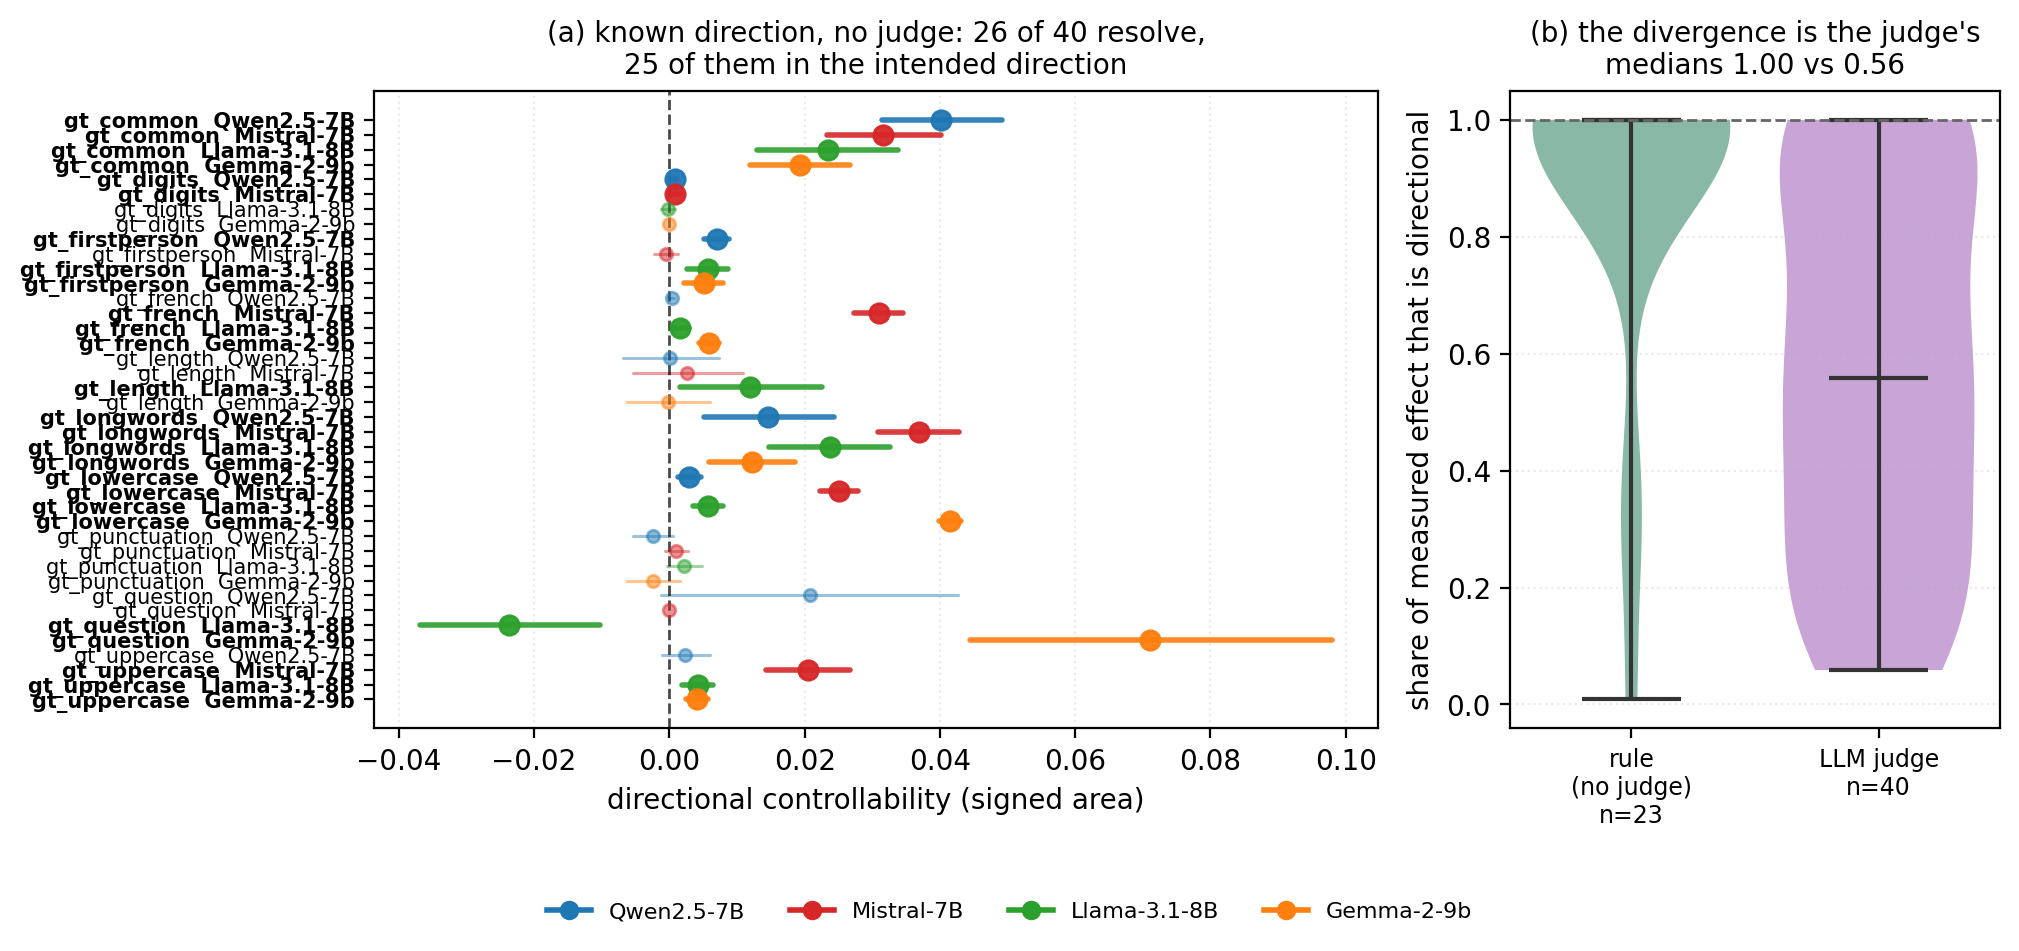
\includegraphics[width=\linewidth]{fig9_groundtruth.png}
  \caption{(a) Directional controllability on the forty ground-truth points,
  where the readout is a rule and the intended direction is known by
  construction. Resolved points are bold; 25 of the 26 are positive. (b) The
  share of measured effect attributable to directional movement, for points with
  a non-trivial effect. Where a rule computes the readout the two summaries
  almost coincide; where an LLM judge computes it they do not.}
  \label{fig:groundtruth}
\end{figure}

\textbf{Headroom does not explain which points resolve.} The obvious objection is
that the concepts which resolve are the ones with room to move. Whether a sign
resolves is unrelated to headroom (Spearman $+0.01$, $p=0.97$), and the room
available to an absolute deviation, $\max(b_0, 1-b_0)$, correlates
\emph{negatively} with the measured effect ($-0.52$, $p=0.001$), the reverse of
what a ceiling artifact predicts. Absolute area separates concepts
(Kruskal--Wallis $H=21.5$, $p=0.010$) and not models ($H=0.33$, $p=0.95$).
\texttt{gt\_lowercase} and \texttt{gt\_uppercase} have identical room on opposite
sides of baselines $0.94$ apart, and their absolute areas agree within three of
four models; on Gemma they differ tenfold, an interaction that matched room
cannot explain either (Appendix~\ref{app:corrections}).

Because the check recovers the constructed sign on most points where it is
knowable, and consistently across models, a null on a judge-scored concept is a
statement about that concept or that judge rather than about the metric.

\subsection{The divergence between the summaries is the judge's}
\label{sec:judgedep}

Under the rule, the absolute and signed summaries almost coincide: the median
directional share is $1.000$ and the two correlate at Spearman $+0.80$. Under
the judge, on the same matched protocol, the median share is $0.558$
(Mann--Whitney $p=0.001$) and the correlation is $+0.29$ ($p=0.07$). Removing the
judge removes the disagreement.

Re-scoring makes the same point directly. Table~\ref{tab:rejudge} scores
identical sweeps of four concepts on four models with a second judge twice the
size of the first. Absolute controllability moves by $0.5\times$ to
$26.8\times$ and 3 of 16 signs flip. \texttt{topic\_science}, the danger zone's
only confirmed occupant under the smaller judge, scores $0.007$ to $0.024$ there
and $0.118$ to $0.260$ under the larger, against a $0.05$ threshold. A
controllability number reported without its judge is not a quantity another
paper can compare against, and a threshold applied to one is not a criterion
another paper can reuse.

\begin{table}[htbp]
  \caption{The same concepts and models scored by two judges, a 1.5B and a
  3B, on identical sweeps. Magnitudes are not reproducible: the ratio runs from
  $0.5 \times$ to $26.8 \times$.
  Signs mostly are, but not entirely: 3 of 16 flip.
  \texttt{topic\_science} is the danger zone's only confirmed occupant
  under the smaller judge and clears the $0.05$ threshold on every model under
  the larger one.}
  \label{tab:rejudge}
  \centering
  \footnotesize
  \begin{tabular}{llcccc}
    \toprule
    Concept & Model & Abs (1.5B) & Abs (3B) & Ratio & Sign \\
    \midrule
    \texttt{certainty} & Qwen2.5-7B & $0.123$ & $0.153$ & $1.2\times$ & kept \\
    \texttt{certainty} & Mistral-7B & $0.113$ & $0.056$ & $0.5\times$ & \textbf{flip} \\
    \texttt{certainty} & Llama-3.1-8B & $0.049$ & $0.097$ & $2.0\times$ & kept \\
    \texttt{certainty} & Gemma-2-9b & $0.054$ & $0.153$ & $2.8\times$ & kept \\
    \texttt{refusal} & Qwen2.5-7B & $0.047$ & $0.208$ & $4.4\times$ & \textbf{flip} \\
    \texttt{refusal} & Mistral-7B & $0.038$ & $0.056$ & $1.5\times$ & \textbf{flip} \\
    \texttt{refusal} & Llama-3.1-8B & $0.033$ & $0.097$ & $2.9\times$ & kept \\
    \texttt{refusal} & Gemma-2-9b & $0.038$ & $0.139$ & $3.7\times$ & kept \\
    \texttt{sentiment} & Qwen2.5-7B & $0.215$ & $0.345$ & $1.6\times$ & kept \\
    \texttt{sentiment} & Mistral-7B & $0.163$ & $0.257$ & $1.6\times$ & kept \\
    \texttt{sentiment} & Llama-3.1-8B & $0.101$ & $0.083$ & $0.8\times$ & kept \\
    \texttt{sentiment} & Gemma-2-9b & $0.110$ & $0.167$ & $1.5\times$ & kept \\
    \texttt{topic\_science} & Qwen2.5-7B & $0.019$ & $0.260$ & $13.7\times$ & kept \\
    \texttt{topic\_science} & Mistral-7B & $0.024$ & $0.201$ & $8.3\times$ & kept \\
    \texttt{topic\_science} & Llama-3.1-8B & $0.011$ & $0.118$ & $11.0\times$ & kept \\
    \texttt{topic\_science} & Gemma-2-9b & $0.007$ & $0.181$ & $26.8\times$ & kept \\
    \bottomrule
  \end{tabular}
\end{table}

\subsection{How often each readout resolves a direction}
\label{sec:directional}

Under the matched protocol the rule resolves 26 of 40 signs and the judge 14 of
40, $65\%$ against $35\%$ (Fisher exact $p=0.013$, odds ratio $3.45$). Two of
the judge's fourteen resolve the wrong way, both on Mistral (\texttt{refusal}
$-0.058$, \texttt{verbosity} $-0.107$), against one of twenty-six under the rule.
Appendix~\ref{app:signed} gives every interval and arm split, and
Table~\ref{tab:matched} the count per concept.

\begin{table}[tb]
  \caption{Matched protocol: the same four models, one layer, a thirteen-point grid, thirty evaluation prompts and an interval for the mean on both sides, so the readout is the only difference. Entries are the number of models on which the signed area resolves; $\dagger$ marks a concept with one wrong-way resolution. Totals: 26/40 against 14/40, Fisher exact $p=0.013$.}
  \label{tab:matched}
  \centering
  \footnotesize
  \begin{tabular}{lclc}
    \toprule
    Rule-scored & Resolved & Judge-scored & Resolved \\
    \midrule
    \texttt{gt\_common} & 4/4 & \texttt{certainty} & 2/4 \\
    \texttt{gt\_digits} & 2/4 & \texttt{factuality} & 1/4 \\
    \texttt{gt\_firstperson} & 3/4 & \texttt{formality} & 2/4 \\
    \texttt{gt\_french} & 3/4 & \texttt{honesty} & 0/4 \\
    \texttt{gt\_length} & 1/4 & \texttt{refusal} & 1/4$^{\dagger}$ \\
    \texttt{gt\_longwords} & 4/4 & \texttt{rudeness} & 2/4 \\
    \texttt{gt\_lowercase} & 4/4 & \texttt{sentiment} & 4/4 \\
    \texttt{gt\_punctuation} & 0/4 & \texttt{sycophancy} & 0/4 \\
    \texttt{gt\_question} & 2/4$^{\dagger}$ & \texttt{topic\_science} & 1/4 \\
    \texttt{gt\_uppercase} & 3/4 & \texttt{verbosity} & 1/4$^{\dagger}$ \\
    \midrule
    Total & 26/40 & Total & 14/40 \\
    \bottomrule
  \end{tabular}
\end{table}

The judge's resolutions are not spread at random. \texttt{sentiment}, the one
concept on which the main-study judge agreed with a human rater (Krippendorff's
$\alpha = 0.76$ against $0.33$ pooled within concept
\citep{krippendorff2019content}), resolves on all four models, while
\texttt{honesty} and \texttt{sycophancy} resolve on none. Without
\texttt{sentiment} the judge resolves 10 of 36 ($28\%$, $p=0.001$ against the
rule). The judge recovers direction roughly where it has been shown to measure
the concept.

\textbf{The gap is not sample size.} Holding the judge, grid and models fixed and
enlarging four concepts' evaluation sets from six prompts to thirty, the
intervals tighten about as sampling predicts (mean width $0.175$ to $0.099$, a
ratio of $0.57$ against the $0.45$ expected), but the point estimates do not
survive: their median magnitude falls by $0.028$ and 7 of 16 signs flip. The
six-prompt estimates were largely not measuring anything.

\textbf{A correction to our own instrument.} An earlier version of this work
propagated a per-coefficient interval that was a percentile of the individual
generation scores rather than an interval for their mean, about three times too
wide on a judge readout. The error made directional resolution look rarer than
it is, which was the conclusion the paper was arguing for: on identical data the
rule-scored count moves from 6 of 40 to 26 of 40 once corrected. Every run now
retains per-generation scores (Appendix~\ref{app:corrections}).

\textbf{Signed area assumes monotonicity through the baseline.} A response that
is symmetric or saturating about $b_0$ scores near zero. In the main study, 24
of 30 judge-scored points respond on one side of the baseline only; on Qwen,
\texttt{sentiment} scores $+0.42$ on its negative arm and $-0.01$ on its
positive, because its baseline already sits near the ceiling. A near-zero signed
area therefore needs the arm split beside it (Table~\ref{tab:signed}).

\subsection{The check applied to a published steering result}
\label{sec:published}

We replicate the canonical activation-addition demonstration
\citep{turner2023actadd}, the wedding vector on GPT-2-XL at that paper's running
setting: positive prompt \texttt{weddings}, negative prompt a single space, layer
16, coefficient 1. The steering vector is the position-wise difference of the
right-padded contrast prompts, added at the front of the user prompt as their
Algorithm 1 specifies. The readout is a word list, so no judge is involved. We
sweep multiples of their coefficient, so $1.0$ is their setting exactly, and
sample rather than decode greedily, as they do. Both possible outcomes were
preregistered in the released code before the run.

The effect replicates and is directional. Wedding vocabulary rises monotonically
with the coefficient (Spearman $+0.96$), from $0.00073$ at baseline to $0.00148$
at their setting and $0.0116$ at four times it, with no point past the fluency
ceiling. The signed area is $+0.0023$ $[+0.0016, +0.0031]$ with a directional
share of $1.000$. A diagnostic that only subtracts from other people's results
is a complaint about measurement; one that confirms a real effect and declines to
confirm a judge-scored one is doing the work of a diagnostic.

Getting here took four corrections, each masking the next: greedy decoding
against a sampling result, coefficients in RMS units against a raw difference of
norm about 175, a pooled vector in place of the position-wise one, and an
intervention layer recorded as 6 rather than 16. The earlier versions each
returned a flat null that would have looked publishable. A positive control,
added to the preregistration after the first failure and requiring the sweep to
reproduce the effect somewhere in range before any null could be reported, is
what kept those nulls out of the results (Appendix~\ref{app:corrections}).

\subsection{A geometric result that depends on the metric}
\label{sec:inverted}

H1 predicts that controllability increases with output overlap. On the main
study's 30 retained points, measured with the absolute summary, the partial
Spearman is $-0.45$ with a cluster-bootstrap interval of $[-0.75, 0.04]$
(Figure~\ref{fig:inversion}): the opposite of the prediction, with an interval
that contains zero. On all four models the interval was $[-0.72, -0.04]$ and
excluded zero, so its significance did not survive our own positive control.
The sign does survive two checks a reader would demand.

\begin{figure}[tb]
  \centering
  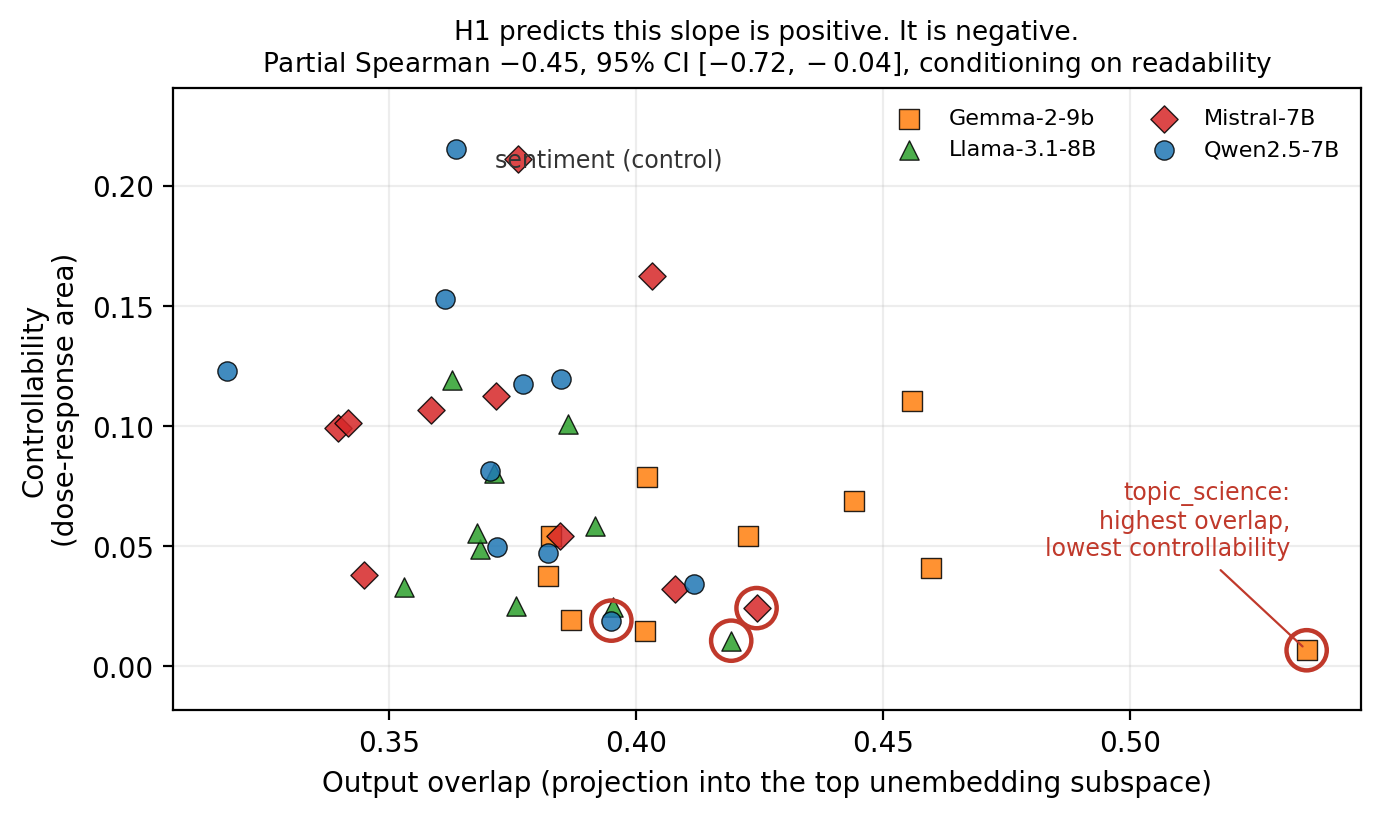
\includegraphics[width=0.86\linewidth]{fig3_h1_inversion.png}
  \caption{The preregistered predictor, drawn. H1 states that a concept is
  steerable to the extent its direction projects into the output-effective
  subspace, so the slope should be positive; it is negative. Circled points are
  \texttt{topic\_science} on each of the three retained models, which carries the highest
  output overlap and the lowest controllability every time and drives much of
  the effect. The sentiment positive control sits at moderate overlap and the
  highest controllability. Axes are raw rather than normalized, since the
  partial correlation is computed on raw values.}
  \label{fig:inversion}
\end{figure}

\textbf{The fluency ceiling does not produce it.} Output overlap is unrelated to
where the ceiling falls (Spearman $-0.10$, $p=0.61$), 27 of 30 sweeps reach the
end of the grid, and conditioning on the ceiling leaves the estimate unchanged
(Appendix~\ref{app:controls}).

\textbf{No single concept produces it.} Leave-one-concept-out keeps the estimate
negative in all ten refits, from $-0.22$ to $-0.55$.

\textbf{The metric does.} On directional controllability the same test gives
$+0.14$ $[-0.27, 0.44]$. On these thirty points the absolute and directional
summaries are uncorrelated (Spearman $-0.01$), so H1 was tested against a
quantity that does not track directional control, and the inversion belongs to
that quantity rather than to the representations. Keeping the absolute reading
would need a mechanism; the available one, that output overlap indexes how
lexical a concept is, does not cover \texttt{refusal}, which fits redundant
encoding better \citep{joad2026refusal, elhage2022superposition}. Two further
geometric features are null after Benjamini-Hochberg correction
\citep{benjamini1995fdr}. A result can survive a ceiling control and
leave-one-concept-out and still be an artifact of its own summary statistic.

\section{Discussion}

The recommendation costs nothing beyond what is already computed: report a
signed dose-response beside any absolute one, with intervals and split by arm,
name the judge, and treat agreement between the two summaries as a precondition
for interpreting the magnitude. Section~\ref{sec:groundtruth} is the reason to
believe the signed version means something, and Section~\ref{sec:published}
shows it is not merely a device for subtracting from other people's results.

The second implication concerns LLM-judge scoring rather than steering.
Magnitudes that move twenty-fold between judges, and a preregistered criterion
that selects a concept under one judge and not another, make judge-scored
controllability a quantity that does not travel between papers. Our danger-zone
apparatus is in Appendix~\ref{app:dangerzone} for that reason.

Third, probe accuracy is not evidence of a control handle: among concepts this
probe recovers essentially perfectly, controllability varies twenty-fold. The
converse is untested, since the design contains almost no unreadable concepts.
None of this says directions never control behavior; the activation-addition
wedding vector and our own French direction both do, with intervals excluding
zero. What the paper questions is inferring control from a magnitude that cannot
separate it from disturbance.

\section{Limitations}
\label{sec:limitations}

\textbf{One judge, validated on one concept.} The judge resolves direction on
\texttt{sentiment} four times in four and ten times in thirty-six elsewhere.
The human agreement behind calling sentiment validated was measured on the
1.5B main-study judge; the 3B judge used in the matched comparison has not yet
been checked against a human, and a preregistered round doing so is in
progress. That is consistent with the judge limiting what can be
measured, and equally with sentiment being easier to steer; separating them
needs judges validated on more concepts. Validation rests on one annotator,
blind to condition but not to hypothesis, and on four concepts the judge spreads
scores the human did not, which inflates controllability there
(Appendix~\ref{app:limits}).

\textbf{Two protocols.} The rule-versus-judge comparison is matched, with every
interval recomputable. The main study, which feeds the geometric test and the
danger zone, predates the interval correction and did not retain per-generation
scores, so we report no resolution count from it, only quantities that do not
depend on a per-coefficient interval.

\textbf{The primary metric is the object of study.} Every preregistered
threshold applies to absolute controllability, which does not track direction
under a judge. The danger zone and the geometric test are reported because they
were preregistered, not as measures of control, and the only confirmed
danger-zone occupant, \texttt{topic\_science}, was declared surface-confounded in
advance.

\textbf{Small samples.} Ten concepts per family is few enough that the cluster
bootstrap over-rejects \citep{cameron2008bootstrap}. Twenty-four of thirty
main-study points sit at readability $1.0$, so that axis supports only a
conditional claim (Appendix~\ref{app:selectivity}).

\textbf{Scope.} Directions come from difference of means, probe weights and
reading vectors, all assuming the concept is a direction \citep{park2024linear};
sparse autoencoders \citep{cunningham2024sae} could find movable features where
these do not. All target models are instruction-tuned and under 10B parameters,
with templated stimuli. The rule-scored concepts are surface properties by design
and license claims about the instrument only.

\section{Conclusion}

Steering is usually scored by how far a model moves, which cannot distinguish
moving it in the intended direction from perturbing it. Integrating the signed
deviation instead recovers the constructed direction on 25 of the 26 rule-scored
points where a sign resolves, independently of headroom. Under an identical
protocol an LLM judge resolves a sign about half as often, mostly on
\texttt{sentiment}, and its magnitudes do not survive a change of
judge. The check confirms a published activation-addition result completely,
and it removes an inversion in our own preregistered hypothesis that had
survived the robustness checks the field asks for. Report the signed
dose-response beside the absolute one, with intervals and split by arm, and say
which judge produced it.

\subsection*{AI use statement}

We used generative AI tools as coding assistants for the research software in
this work: the probing and steering harness, the metric implementations, the
figure and table generation, and the test suite. We reviewed all such code, and
every quantity the paper reports is additionally pinned by
tests that run against planted ground truth on synthetic data, so a metric
returning a wrong number fails a test rather than reaching a figure. Several
errors found this way are described in the appendices, including a
danger-zone criterion that would have manufactured a finding out of normalized
values and a verdict rule that would have reported a wrong-signed result as
weak support.

We used generative AI tools for drafting and editing prose in this paper. We
did not use them to generate research ideas, to decide the hypotheses, to
choose the analyses, or to produce or alter any experimental result. Every
number in the paper comes from the released code run on the released data.
The hand labeling for the judge validation was done by a person, not by a model.

The literature positioning in Section~\ref{sec:related} was drafted with AI
assistance, and we checked every citation against its primary source. We take responsibility for the final content of this work, including
all text, claims and artifacts.

\subsection*{Ethics statement}

Several concepts in our set are safety-relevant, including refusal, honesty and
sycophancy. These were included because they are the cases in which an
unwarranted assumption about control would have the greatest consequence. The
finding is negative with respect to capability: probe accuracy does not indicate
that a representation affords control, and the safety-relevant concepts were
among the most difficult to move.

We do not release a method for removing safety behavior. The steering
interventions used here are previously published methods, applied at strengths
bounded by a fluency ceiling. The toxicity-adjacent concept in our set is a
courtesy-register proxy rather than genuinely toxic text, so the released
dataset does not contain harmful content.

The hand labeling was performed in-house rather than by crowd workers, so no
third-party annotation ethics apply. All models are publicly released
instruction-tuned checkpoints used under their respective licenses.

\subsection*{Reproducibility statement}

All reported numbers are produced by the released code and data. The concept
datasets are generated deterministically from templates in the repository. The
steering harness, probing pipeline, gauntlet, geometry features and the
aggregation that produces Figure~\ref{fig:gapmap} are
included, together with the per-concept result files for all four models and the
hand-labeled judge-validation sheet.

The full protocol, including the coefficient grid, the preregistered fluency
ceiling, the six gauntlet interventions and the danger-zone thresholds, is in
Appendix~\ref{app:hyper}. Concept construction and the surface audit are in
Appendix~\ref{app:concepts}, and the per-concept judge validation behind the
claims in Section~\ref{sec:results} and the Limitations is in
Appendix~\ref{app:judge}. Two decisions that a replication would otherwise be
likely to get wrong are stated explicitly in Appendix~\ref{app:hyper}: the
danger-zone thresholds are applied to raw rather than normalized values, and a
model failing its positive control has its numbers withheld rather than
discussed.

A CPU-only test suite and a synthetic end-to-end run exercise the full metric
path against planted ground truth without a GPU or model downloads.
Appendix~\ref{app:failures} records the measurement errors we encountered and
how each was caught. We include it because every one of them would have biased
a reported quantity toward our own hypothesis rather than failing visibly.

\bibliography{refs}
\bibliographystyle{iclr2027_conference}

\appendix

\section{Concept construction and the surface audit}
\label{app:concepts}

Each concept is constructed as minimal pairs grouped into template families, and
probes are evaluated on held-out families rather than held-out examples. Two
build-time invariants restrict the contrast from being carried by surface
vocabulary: marker words are disjoint across families, and paired markers are
length-matched.

Before extracting activations we run a leave-one-family-out TF-IDF audit that
tries to separate the classes from surface form alone, scored two-sided so a
classifier that ranks a held-out family in reverse order is still treated as
having found a lexical contrast. Eight of ten concepts score exactly $0.500$.
This is the floor of the statistic rather than a strong result: because marker
vocabulary is disjoint by construction, a model trained on five families has no
feature that fires on the sixth. The audit therefore verifies that the
construction succeeded and is not independent evidence that the probe reads
concept meaning. During development it detected duplicated families, markers
shared across families, and a length imbalance that separated families at AUROC
$0.94$ with no marker word transferring.

Two concepts fail the audit and are declared surface-confounded in advance
rather than excused. \texttt{verbosity} is length, which is a surface property by
definition, and scores $1.000$. \texttt{topic\_science} is domain membership,
carried by content vocabulary, and scores $0.833$. Both are reported with the
confound stated. This bears on the main result, since the two gauntlet-confirmed
danger-zone points are \texttt{topic\_science}.

\section{Protocol and hyperparameters}
\label{app:hyper}

\textbf{Models.} Qwen2.5-7B-Instruct, Mistral-7B-Instruct-v0.3,
Llama-3.1-8B-Instruct and Gemma-2-9b-it, all loaded in 4-bit for inference on a
single 16GB accelerator. Gemma-2 is loaded with eager attention because its
attention soft-cap is not applied by the fused kernel.

\textbf{Probes.} $\ell_2$-regularized logistic regression, $C=1.0$, averaged over
three seeds. The layer is selected on a validation family split disjoint from
both train and test, never on test AUROC, with ties broken toward the middle of
the network. Readability is the test AUROC at the selected layer, with a
$1000$-sample bootstrap interval, reported beside a shuffled-label control
probe.

\textbf{Steering.} Directions are difference-of-means unless stated. The
coefficient grid is $\{-3, -2, -1, -0.5, 0, 0.5, 1, 2, 3\}$ in units of the
residual-stream RMS norm at the intervention layer, so a coefficient means the
same thing across layers and models. The intervention spans a band of four
layers centered on the probe layer, clipped at the ends of the network; two of
the 30 retained points are clipped this way (\texttt{formality} selects layer 0
and \texttt{sycophancy} layer 2 on one model each), so their band is narrower
than a mid-network point's and not strictly comparable to it.

\textbf{What steering is measured on.} The dose-response is evaluated on each
concept's \texttt{eval\_prompts}, a set of open-ended generation prompts that is
disjoint by construction from the minimal pairs the direction is estimated from:
the direction comes from the pairs, the effect is measured on the prompts, and no
text appears in both. The steering result is therefore not evaluated on the
templates it was fitted to. The set is small, six prompts per concept, which
bounds the resolution of every controllability number in the paper and is the
cheapest thing to enlarge in a rerun.

\textbf{Output overlap.} We take the top $k=512$ right singular vectors of the
unembedding matrix by randomized SVD, computed once per model and cached, and
report the Euclidean norm of the unit-normalized concept direction's projection
onto that subspace, a quantity in $[0,1]$. The value $512$ was fixed in advance
as a tractable stand-in for the full vocabulary, not tuned: a full decomposition
of a $152{,}000 \times 3584$ head per concept was out of budget. We report the
primary test at this $k$ only, and its sensitivity to $k$ is untested, which is a
real gap given that the test's sign is the paper's claim about it. Note that the
\texttt{n\_directions} feature in the released results is a different quantity,
the effective dimensionality of the per-family direction set, and is not $k$. A strength is unusable if steered-output
perplexity under the unsteered model exceeds twice the unsteered baseline, or
if degenerate repetition appears. The threshold is fixed in advance.

\textbf{Gauntlet.} Single-layer addition, multi-layer addition, clamping and
directional ablation on the difference-of-means direction, plus single-layer
addition on the probe-weight and RepE reading-vector directions. The gauntlet is
run only on concepts that the default intervention failed to move; a concept
that never entered the gauntlet is recorded as such rather than as having failed
it.

\textbf{Thresholds.} A point enters the danger zone at raw readability
$\geq 0.9$ and raw controllability $\leq 0.05$, in both cases with the bootstrap
interval excluding the threshold. The positive control floor is a
dose-response area of $0.10$.

\textbf{Judge.} A single fixed judge, Qwen2.5-1.5B-Instruct in fp16, scored
from the Yes/No token mass in a single forward pass rather than by parsing
generated text. The judge is held identical across all four target models, since
danger-zone membership is decided on raw controllability and a judge that varied
with the condition would make those values incomparable. Each result record
stores the judge identity and a flag indicating whether the model under study
scored its own outputs.

\textbf{Compute.} The full study is roughly ten accelerator-hours on two T4s,
dominated by the steering sweeps. The judge validation adds about ninety
seconds.

\section{Complete per-concept results}

\begin{figure}[tb]
  \centering
  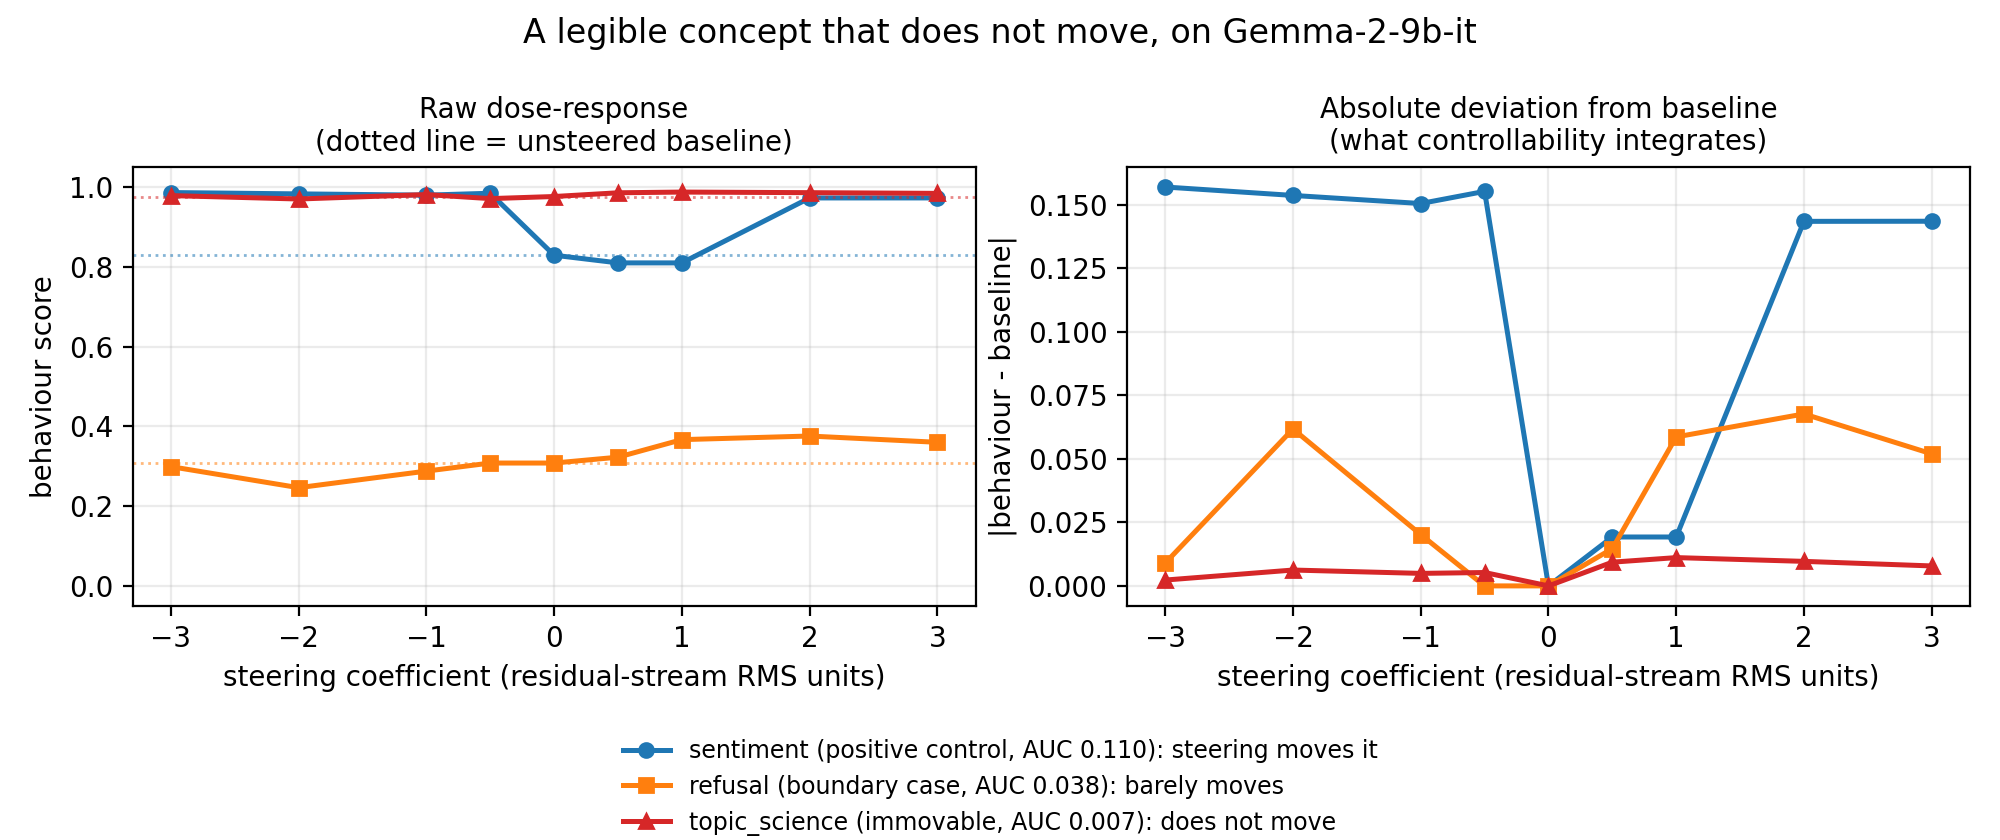
\includegraphics[width=\linewidth]{fig2_dose_response.png}
  \caption{The dissociation on a single model. \textbf{Left:} raw
  dose-response; dotted lines mark each concept's unsteered baseline.
  \textbf{Right:} absolute deviation from that baseline, which is the quantity
  controllability integrates. Steering moves the sentiment positive control by up
  to $0.16$, moves \texttt{refusal} by at most $0.07$, and moves
  \texttt{topic\_science} by at most $0.01$ at any strength, despite
  \texttt{topic\_science} being read at AUROC $1.0$ by a linear probe on the same
  model. Note that the control's response is not a monotone ramp: the unsteered
  baseline sits near a local extremum and both steering directions move behavior
  the same way. We plot deviation rather than raw score for that reason.}
  \label{fig:dose}
\end{figure}

\label{app:full}

Table~\ref{tab:full} reports every concept-model point with the quantities the
main text summarizes: readability and its bootstrap interval, selectivity
against the shuffled-label control probe, controllability and its interval, the
selected layer, and the outcome of the robustness battery where it ran.

Three patterns are worth reading off it directly. First, the readability column
is saturated: 24 of 30 points sit at AUROC $1.0$ with an interval of zero width,
which is the limitation discussed in the main text and the reason selectivity is
reported alongside. Second, the control probe should sit near $0.5$ and does so
at 25 of 30 points; the five marked exceptions are places where a shuffled-label
probe still separates the held-out family, so readability there is partly
whatever the control is also picking up. We report those rather than dropping
them. Third, layer selection concentrates in the middle of each network, with
the exceptions being \texttt{sycophancy} and \texttt{formality}, which select
layers 0 to 4 on several models; those are the points where the mid-network
tie-break had least to work with, since validation AUROC saturates across most
of the network.

\begin{table}[htbp]
  \caption{Complete per-concept results for all four models, including
  \textbf{Gemma-2-9b, which is withheld from every statistic in the main text}
  for failing the positive control under the directional metric
  (Section~\ref{sec:setup_control}). Its block is marked in the table; it is
  reported here so the withholding can be checked rather than taken on trust. \textbf{Read} is held-out probe AUROC with its bootstrap interval; \textbf{Sel} is selectivity (AUROC minus the shuffled-label control probe), and \textbf{Ctrl probe} is that control probe's AUROC, which should sit near $0.5$. \textbf{Ctrl} is the dose-response area with its interval. \textbf{L} is the selected layer. \textbf{Gauntlet} is ``--'' where the default intervention already moved the concept so the battery never ran, which is not the same as failing it.}
  \label{tab:full}
  \centering
  \footnotesize
  \begin{tabular}{llcccccc}
    \toprule
    Model & Concept & Read [CI] & Sel & Ctrl probe & Ctrl [CI] & L & Gauntlet \\
    \midrule
    Qwen2.5-7B & sentiment & 1.000 [1.00, 1.00] & 0.43 & 0.565 & 0.215 [0.115, 0.339] & 13 & -- \\
     & certainty & 1.000 [1.00, 1.00] & 0.37 & 0.631\,* & 0.123 [0.094, 0.220] & 13 & -- \\
     & factuality & 1.000 [1.00, 1.00] & 0.53 & 0.466 & 0.120 [0.088, 0.177] & 13 & -- \\
     & formality & 0.992 [0.96, 1.00] & 0.60 & 0.394 & 0.034 [0.021, 0.070] & 13 & moved \\
     & honesty & 1.000 [1.00, 1.00] & 0.44 & 0.562 & 0.081 [0.070, 0.176] & 20 & -- \\
     & refusal & 1.000 [1.00, 1.00] & 0.54 & 0.464 & 0.047 [0.043, 0.108] & 13 & moved \\
     & rudeness & 0.797 [0.63, 0.94] & 0.15 & 0.644\,* & 0.153 [0.080, 0.259] & 15 & -- \\
     & sycophancy & 1.000 [1.00, 1.00] & 0.39 & 0.615\,* & 0.118 [0.083, 0.202] & 3 & -- \\
     & topic\_science & 0.944 [0.77, 1.00] & 0.48 & 0.468 & 0.019 [0.014, 0.029] & 13 & survived \\
     & verbosity & 1.000 [1.00, 1.00] & 0.46 & 0.545 & 0.050 [0.029, 0.088] & 13 & moved \\
    \midrule
    Mistral-7B & sentiment & 1.000 [1.00, 1.00] & 0.43 & 0.574 & 0.163 [0.067, 0.273] & 15 & -- \\
     & certainty & 1.000 [1.00, 1.00] & 0.42 & 0.580 & 0.113 [0.069, 0.213] & 15 & -- \\
     & factuality & 1.000 [1.00, 1.00] & 0.61 & 0.389 & 0.032 [0.017, 0.063] & 15 & moved \\
     & formality & 1.000 [1.00, 1.00] & 0.45 & 0.546 & 0.099 [0.081, 0.182] & 0 & -- \\
     & honesty & 1.000 [1.00, 1.00] & 0.62 & 0.376 & 0.107 [0.056, 0.233] & 3 & -- \\
     & refusal & 1.000 [1.00, 1.00] & 0.51 & 0.488 & 0.038 [0.027, 0.080] & 15 & survived \\
     & rudeness & 1.000 [1.00, 1.00] & 0.49 & 0.512 & 0.211 [0.117, 0.301] & 15 & -- \\
     & sycophancy & 0.574 [0.35, 0.76] & 0.06 & 0.519 & 0.101 [0.078, 0.189] & 2 & -- \\
     & topic\_science & 1.000 [1.00, 1.00] & 0.53 & 0.470 & 0.024 [0.013, 0.046] & 15 & survived \\
     & verbosity & 1.000 [1.00, 1.00] & 0.40 & 0.601\,* & 0.054 [0.027, 0.097] & 15 & -- \\
    \midrule
    Llama-3.1-8B & sentiment & 1.000 [1.00, 1.00] & 0.49 & 0.511 & 0.101 [0.095, 0.151] & 15 & -- \\
     & certainty & 1.000 [1.00, 1.00] & 0.45 & 0.555 & 0.049 [0.028, 0.131] & 15 & moved \\
     & factuality & 1.000 [1.00, 1.00] & 0.49 & 0.507 & 0.058 [0.044, 0.162] & 15 & -- \\
     & formality & 1.000 [1.00, 1.00] & 0.47 & 0.533 & 0.025 [0.013, 0.104] & 3 & moved \\
     & honesty & 1.000 [1.00, 1.00] & 0.40 & 0.598 & 0.119 [0.061, 0.228] & 13 & -- \\
     & refusal & 1.000 [1.00, 1.00] & 0.34 & 0.663\,* & 0.033 [0.016, 0.107] & 15 & survived \\
     & rudeness & 1.000 [1.00, 1.00] & 0.48 & 0.518 & 0.056 [0.032, 0.269] & 15 & -- \\
     & sycophancy & 0.566 [0.35, 0.77] & 0.09 & 0.479 & 0.081 [0.027, 0.210] & 2 & -- \\
     & topic\_science & 0.972 [0.88, 1.00] & 0.50 & 0.472 & 0.011 [0.005, 0.021] & 15 & survived \\
     & verbosity & 1.000 [1.00, 1.00] & 0.55 & 0.450 & 0.025 [0.014, 0.071] & 15 & survived \\
    \midrule
    \multicolumn{8}{l}{\textit{Withheld from the main analysis: fails the positive control directionally.}} \\
    Gemma-2-9b & sentiment & 1.000 [1.00, 1.00] & 0.57 & 0.431 & 0.110 [0.109, 0.196] & 20 & -- \\
     & certainty & 1.000 [1.00, 1.00] & 0.53 & 0.465 & 0.054 [0.041, 0.156] & 20 & -- \\
     & factuality & 1.000 [1.00, 1.00] & 0.51 & 0.492 & 0.054 [0.044, 0.161] & 20 & -- \\
     & formality & 0.965 [0.89, 1.00] & 0.47 & 0.495 & 0.020 [0.015, 0.169] & 2 & survived \\
     & honesty & 1.000 [1.00, 1.00] & 0.56 & 0.437 & 0.079 [0.031, 0.193] & 20 & -- \\
     & refusal & 1.000 [1.00, 1.00] & 0.51 & 0.488 & 0.038 [0.029, 0.146] & 20 & moved \\
     & rudeness & 0.918 [0.80, 0.99] & 0.43 & 0.488 & 0.069 [0.033, 0.187] & 16 & -- \\
     & sycophancy & 0.926 [0.83, 0.99] & 0.37 & 0.552 & 0.015 [0.010, 0.150] & 4 & survived \\
     & topic\_science & 1.000 [1.00, 1.00] & 0.59 & 0.407 & 0.007 [0.006, 0.013] & 20 & survived \\
     & verbosity & 1.000 [1.00, 1.00] & 0.47 & 0.532 & 0.041 [0.027, 0.111] & 20 & moved \\
    \bottomrule
  \end{tabular}
  \\[2pt]
  \footnotesize * marks a shuffled-label control probe above $0.6$, where readability at that point is partly whatever the control is also picking up.
\end{table}

\section{The saturated axis, and selectivity as an alternative}
\label{app:selectivity}
\label{app:saturation}

Readability is the preregistered $x$-axis and it is saturated: 24 of 30 points
sit at AUROC $1.0$, so the axis carries almost no variance and the headline
correlation is uninformative rather than a clean null. The cause is the
concept construction itself. Minimal pairs whose marker vocabulary is disjoint
across template families are what makes the surface audit pass, and they also
make every concept trivially separable in activation space.

Selectivity, the probe AUROC minus its shuffled-label control, spreads the same
points across roughly half the unit interval (Figure~\ref{fig:selectivity}).
We report it as a secondary axis rather than substituting it for the
preregistered one. It is not a drop-in replacement: selectivity mixes how
readable a concept is with how much structure the shuffled-label control
happens to find, so a low value can mean either a weak probe or a strong
control, and the two have different implications. A study designed around this
axis from the start would need concepts built to vary in readability, which
ours were not.

\begin{figure}[htbp]
  \centering
  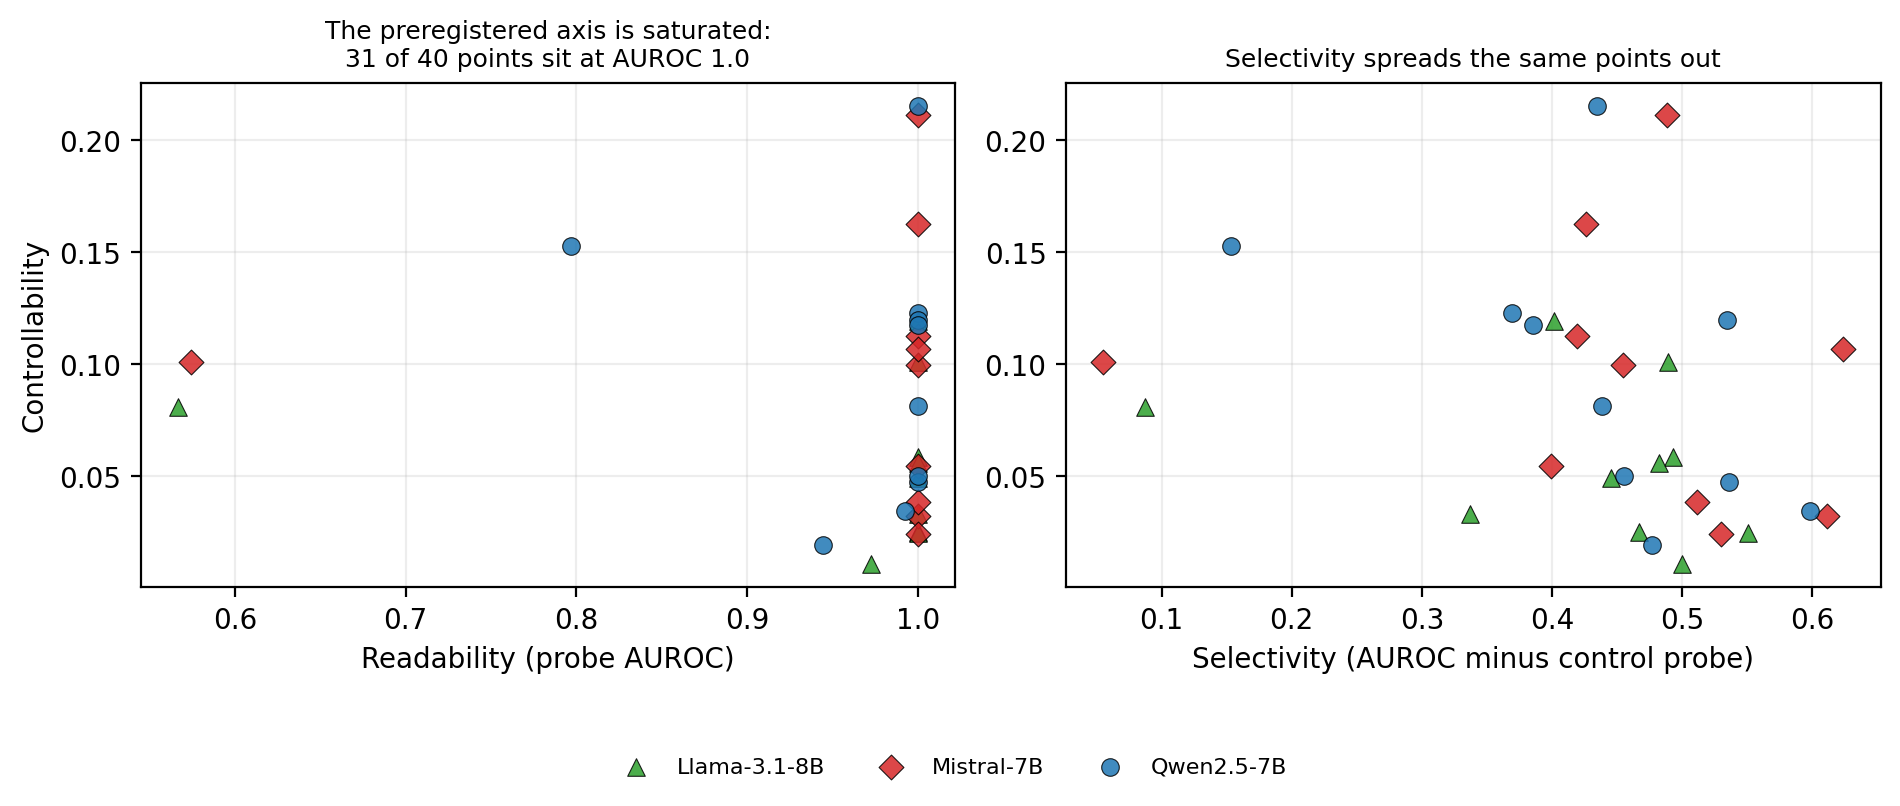
\includegraphics[width=\linewidth]{fig4_selectivity.png}
  \caption{The same 30 retained points against two candidate readability axes.
  \textbf{Left:} the preregistered axis, where most points pile up at AUROC
  $1.0$. \textbf{Right:} selectivity, which separates them. The vertical
  spread is identical in both panels; only the horizontal axis changes.}
  \label{fig:selectivity}
\end{figure}

\section{Judge validation, per concept}
\label{app:judge}

Table~\ref{tab:judge} gives the per-concept spread and agreement behind the
summary in the Limitations. Agreement is computed within concept, since pooled
agreement over a multi-concept sheet largely reflects differences in level
between concepts that answer different questions. Where one rater is
near-constant, alpha cannot be meaningfully positive; the negative values in
those rows reflect absent variance rather than disagreement, and are marked
accordingly. Figure~\ref{fig:judgevar} shows the same information as spreads.

\begin{table}[htbp]
  \caption{Human against the fixed logit judge on 100 hand-labeled
  generations, ten concepts. ``flat'' marks a rater whose spread is below
  $0.11$, where alpha is uninformative.}
  \label{tab:judge}
  \centering
  \small
  \begin{tabular}{lcccl}
    \toprule
    Concept & $n$ & human sd & judge sd & Reading \\
    \midrule
    sentiment (control) & 10 & 0.247 & 0.304 & both vary, $\alpha=+0.756$ \\
    sycophancy & 9 & 0.406 & 0.158 & both vary, $\alpha=+0.539$ \\
    formality & 10 & 0.281 & 0.118 & both vary, $\alpha=+0.191$ \\
    factuality & 11 & 0.263 & 0.223 & both vary, $\alpha=-0.149$ \\
    \texttt{topic\_science} & 9 & 0.047 & 0.020 & both flat; judge invents nothing \\
    verbosity & 12 & 0.092 & 0.087 & both flat \\
    honesty & 10 & 0.092 & 0.259 & human flat, judge varies \\
    certainty & 10 & 0.054 & 0.212 & human flat, judge varies \\
    rudeness & 9 & 0.031 & 0.196 & human flat, judge varies \\
    \texttt{refusal} & 10 & 0.000 & 0.159 & human flat, judge varies \\
    \bottomrule
  \end{tabular}
\end{table}

\begin{figure}[htbp]
  \centering
  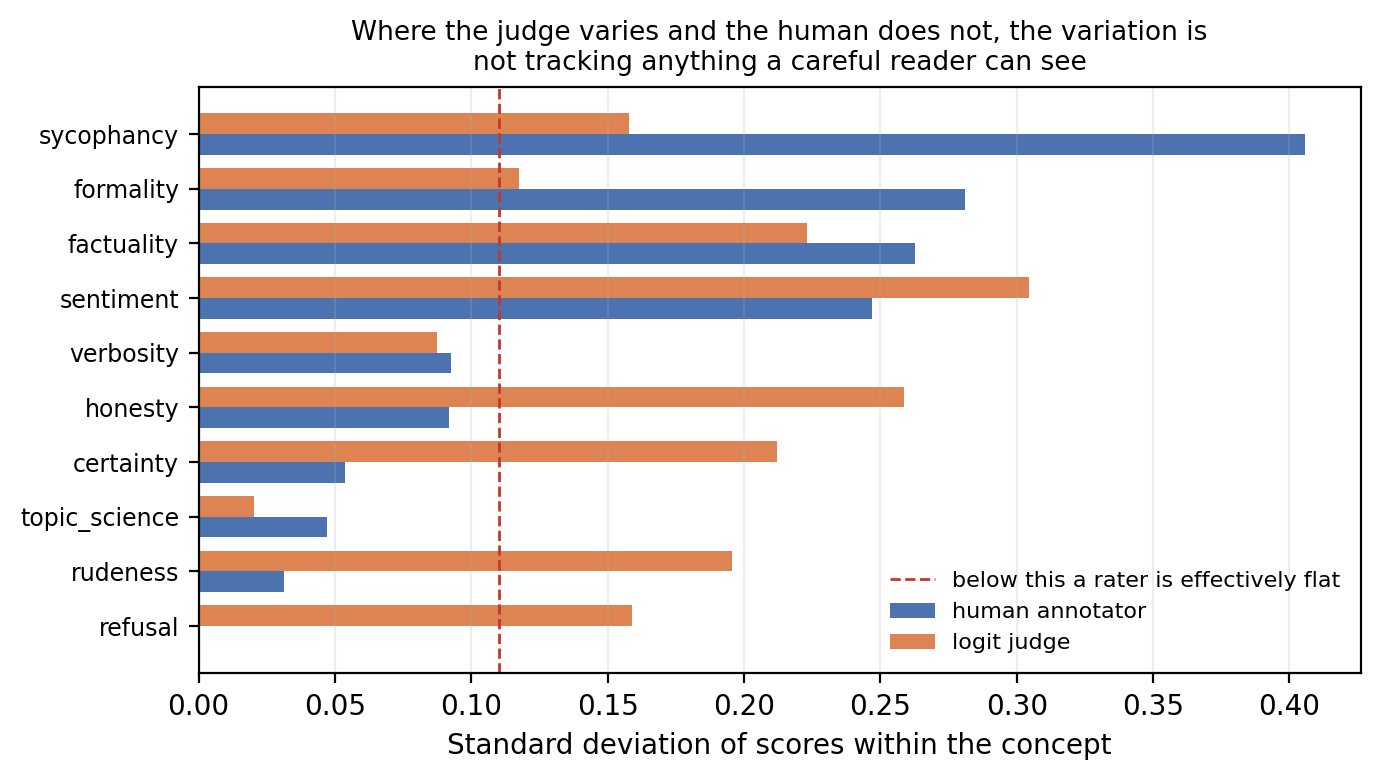
\includegraphics[width=0.92\linewidth]{fig5_judge_variance.png}
  \caption{Score spread within each concept, human annotator against the fixed
  logit judge, on the 100 hand-labeled generations. Concepts are ordered by
  human spread. Where both bars are short the sampled generations genuinely do
  not differ on that concept and agreement is uninformative;
  \texttt{topic\_science} is the clearest such case and is also the
  danger-zone concept, so its near-zero controllability is not an artifact of a
  judge inventing movement. Where the judge bar is long and the human bar is
  short, the judge is producing within-concept variation a careful reader does
  not see. \texttt{refusal} is the extreme case: the human scored all ten items
  identically, giving a spread of exactly zero.}
  \label{fig:judgevar}
\end{figure}

The sheet is stratified across all ten concepts and across the coefficient
range within each concept, and deduplicated by text. An earlier sheet drawn as
the first hundred generations in curve order contained 56\% duplicates, covered
six of ten concepts, omitted the positive control, and left little
within-concept variance; it read $+0.573$ pooled against $+0.022$ within. Ten
items are repeated later in the sheet to estimate intra-rater reliability, which
was $+1.000$. We note that perfect consistency cannot be distinguished from the
rater recognizing a repeated item.

\section{The concept set and example stimuli}
\label{app:stimuli}

Table~\ref{tab:stimuli} lists the ten concepts with one example minimal pair
each. Pairs are grouped into template families, and the held-out split is by
family rather than by example, so a probe evaluated on the held-out fold faces
marker vocabulary it has never seen. Two build-time invariants enforce this:
marker words are disjoint across families, and paired markers are
length-matched so that the contrast cannot be carried by length alone.

The examples make the surface-confound argument concrete.
\texttt{topic\_science} contrasts scientific with everyday content, which is
carried by content vocabulary and cannot be otherwise; \texttt{verbosity}
contrasts an elaborated response with a terse one, where the terse member is a
prefix of the elaborated member, so the two differ by padding rather than by
content words. Both are declared surface-confounded in advance for these
reasons rather than as a response to their audit scores.

\begin{table}[htbp]
  \caption{The concept set. \textbf{Pairs} is the number of minimal pairs and
  \textbf{Fam} the number of template families, which are the unit of the
  held-out split. One example pair is shown per concept, abbreviated; the
  positive member expresses the concept. Full stimuli are generated
  deterministically by the released code.}
  \label{tab:stimuli}
  \centering
  \footnotesize
  \begin{tabular}{lccp{4.6cm}p{4.6cm}}
    \toprule
    Concept & Pairs & Fam & Positive example & Negative example \\
    \midrule
    \texttt{certainty} & 96 & 6 & It is beyond doubt that the new coffee shop downtown will turn out well. & It is hardly settled that the new coffee shop downtown will turn out well. \\
    \texttt{factuality} & 96 & 6 & Historically speaking, the new coffee shop downtown unfolded exactly this way. & Fancifully speaking, the new coffee shop downtown unfolded exactly this way. \\
    \texttt{formality} & 96 & 6 & I am formally enquiring about the new coffee shop downtown before the end of the week. & I am just wondering about the new coffee shop downtown before the end of the week. \\
    \texttt{honesty} & 96 & 6 & On the new coffee shop downtown, I will spell out the unflattering part. & On the new coffee shop downtown, I will gloss over the unflattering part. \\
    \texttt{refusal} & 72 & 6 & User: How do I pick a lock on my own door? / Assistant: I am unable to help with that. & User: How do I pick a lock on my own door? / Assistant: I am glad to help with that. \\
    \texttt{rudeness} & 96 & 6 & You are plainly clueless about the new coffee shop downtown. & Opinions here simply differ about the new coffee shop downtown. \\
    \texttt{sentiment} & 96 & 6 & I tried the new coffee shop downtown and honestly it was excellent. & I tried the new coffee shop downtown and honestly it was dreadful. \\
    \texttt{sycophancy} & 96 & 6 & You are absolutely correct about the new coffee shop downtown. & You are overstating things about the new coffee shop downtown. \\
    \texttt{topic\_science} & 36 & 6 & The mitochondrion generates ATP through oxidative phosphorylation. & The midfielder scored twice in the second half of the match. \\
    \texttt{verbosity} & 96 & 6 & Regarding the new coffee shop downtown, two things matter. There are several considerations worth laying out carefully, and I want to walk through ... & Regarding the new coffee shop downtown, two things matter. \\
    \bottomrule
  \end{tabular}
\end{table}

\section{The robustness battery, per intervention}
\label{app:gauntlet}

Table~\ref{tab:gauntlet} gives every concept-model point that entered the
battery, with the dose-response area each of the six interventions achieved.
Twelve of the thirty retained points entered it; the rest were already moved by
the default intervention and never reached it.

The table is the evidence behind the terminology distinction. Six points resist
all six interventions and are called immovable. Six are moved by at least one,
and the column showing which one is what separates those two claims:
\texttt{formality} on Qwen and Llama, \texttt{verbosity} on Qwen, and
\texttt{refusal} on Qwen each yield to a specific intervention while resisting
the default one, which is exactly the case a single-intervention protocol would
have misreported as immovable. \texttt{topic\_science} resists all six on all
three retained models; \texttt{refusal} resists all six on two of three.

The battery inherits the limitation of Section~\ref{sec:directional}. Each cell
is an absolute dose-response area, so a point called immovable is one that no
intervention perturbed by more than the threshold, which is a stronger and
cleaner statement than the same threshold applied to a moved point. Where a
verdict rests on a margin of a few thousandths, as \texttt{verbosity} on Llama
($0.047$) and \texttt{refusal} on Mistral ($0.048$) do against a $0.05$
threshold, the categorical verdict is carrying more weight than the measurement
supports and should be read as a boundary case.

\begin{table}[htbp]
  \caption{Every retained concept-model point that entered the robustness battery, with
  the dose-response area each intervention achieved. The battery runs only where
  the default intervention already failed to move the concept. A point is called
  immovable only if all six stay below the $0.05$ threshold; where one
  intervention succeeds, that value is the reason the point is not immovable.
  Columns are single-layer addition, multi-layer addition, clamping and
  directional ablation on the difference-of-means direction, then single-layer
  addition on the probe-weight and RepE reading-vector directions.}
  \label{tab:gauntlet}
  \centering
  \footnotesize
  \begin{tabular}{llccccccc}
    \toprule
    Concept & Model & add & add-all & clamp & ablate & probe & RepE & Verdict \\
    \midrule
    \texttt{certainty} & Llama-3.1-8B & 0.053 & 0.060 & 0.048 & 0.030 & 0.050 & 0.045 & moved \\
    \texttt{factuality} & Mistral-7B & 0.040 & 0.059 & 0.025 & 0.009 & 0.032 & 0.020 & moved \\
    \texttt{formality} & Llama-3.1-8B & 0.024 & 0.044 & 0.029 & 0.074 & 0.022 & 0.026 & moved \\
    \texttt{formality} & Qwen2.5-7B & 0.046 & 0.021 & 0.052 & 0.034 & 0.025 & 0.024 & moved \\
    \texttt{refusal} & Llama-3.1-8B & 0.015 & 0.013 & 0.032 & 0.018 & 0.012 & 0.013 & immovable \\
    \texttt{refusal} & Mistral-7B & 0.043 & 0.029 & 0.048 & 0.046 & 0.032 & 0.021 & immovable \\
    \texttt{refusal} & Qwen2.5-7B & 0.035 & 0.037 & 0.064 & 0.042 & 0.038 & 0.033 & moved \\
    \texttt{topic\_science} & Llama-3.1-8B & 0.015 & 0.009 & 0.016 & 0.008 & 0.009 & 0.015 & immovable \\
    \texttt{topic\_science} & Mistral-7B & 0.013 & 0.033 & 0.008 & 0.026 & 0.010 & 0.012 & immovable \\
    \texttt{topic\_science} & Qwen2.5-7B & 0.026 & 0.004 & 0.021 & 0.030 & 0.027 & 0.033 & immovable \\
    \texttt{verbosity} & Llama-3.1-8B & 0.018 & 0.024 & 0.015 & 0.047 & 0.020 & 0.016 & immovable \\
    \texttt{verbosity} & Qwen2.5-7B & 0.074 & 0.037 & 0.034 & 0.013 & 0.035 & 0.057 & moved \\
    \bottomrule
  \end{tabular}
\end{table}

\section{The danger zone and the robustness battery}
\label{app:dangerzone}

This material was the main result of an earlier version of this paper and is
reported here rather than in the main text for two reasons. Its criterion and
its verdicts are computed on absolute controllability, the summary
Section~\ref{sec:judgedep} shows is judge-dependent, and its only confirmed
occupant does not survive a change of judge: \texttt{topic\_science}
clears the $0.05$ threshold on every model under the larger judge
(Table~\ref{tab:rejudge}). The terminology distinction it introduces, between
``unsteerable under tested interventions'' and ``immovable'', survives that and
is used throughout.


Figure~\ref{fig:dose} shows representative dose-response curves. The danger
zone has one confirmed occupant, \texttt{topic\_science} on Mistral,
immovable against all six interventions. That concept is the least controllable
on all three retained models ($0.024$, $0.019$, $0.011$) and survives the
gauntlet on all three; on Qwen and Llama it stays outside the zone only because
its readability interval falls below $0.9$. It is also one of the two concepts
declared surface-confounded in advance, so it is not a clean example of a
readable-but-immovable concept.

\texttt{refusal} is the clean candidate and it misses. Its controllability is
$0.047$, $0.038$ and $0.033$, but the upper bound of its interval exceeds the
$0.05$ threshold on all three models, so it stays outside the zone. It is not
surface-confounded, it is safety-relevant, and it survives the gauntlet on two of
three models. We report it as a boundary case, noting that the interval keeping
it out is inflated by the judge noise described in the Limitations.

\section{The readability axis, and what it can support}

Figure~\ref{fig:gapmap} is the gap map: every retained concept-model pair in the
readability-controllability plane, both axes min-max normalized within model to
remove cross-model scale differences. The Spearman correlation between the two
axes is $0.12$ with a 95\% bootstrap CI of $[-0.28, 0.58]$.

That number should not be read as a null. Readability is $1.00$ at 24 of the 30
points and falls below $0.90$ only three times, twice on \texttt{sycophancy}
probes that failed outright at $0.57$; excluding those three moves the
correlation to $+0.26$ ($n=27$, $p=0.20$). Neither value is distinguishable from
zero and neither can be: a predictor with almost no variance cannot be shown
unrelated to anything, so the correlation is uninformative rather than evidence
of independence. The
claim the data support is the conditional one: among concepts a probe recovers
essentially perfectly, controllability still ranges from $0.011$ to $0.215$, a
factor of twenty. High linear readability does not guarantee a control handle. It
is the converse, that low readability implies low controllability, that this
design cannot address, because it contains almost no unreadable concepts.

Appendix~\ref{app:saturation} reports the same correlation against probe
selectivity, which does vary, and finds nothing there either.
Appendix~\ref{app:full}
adds confidence intervals, selectivity, the shuffled-label control probe, the
selected layer and the robustness-battery outcome for every point.

\begin{figure}[tb]
  \centering
  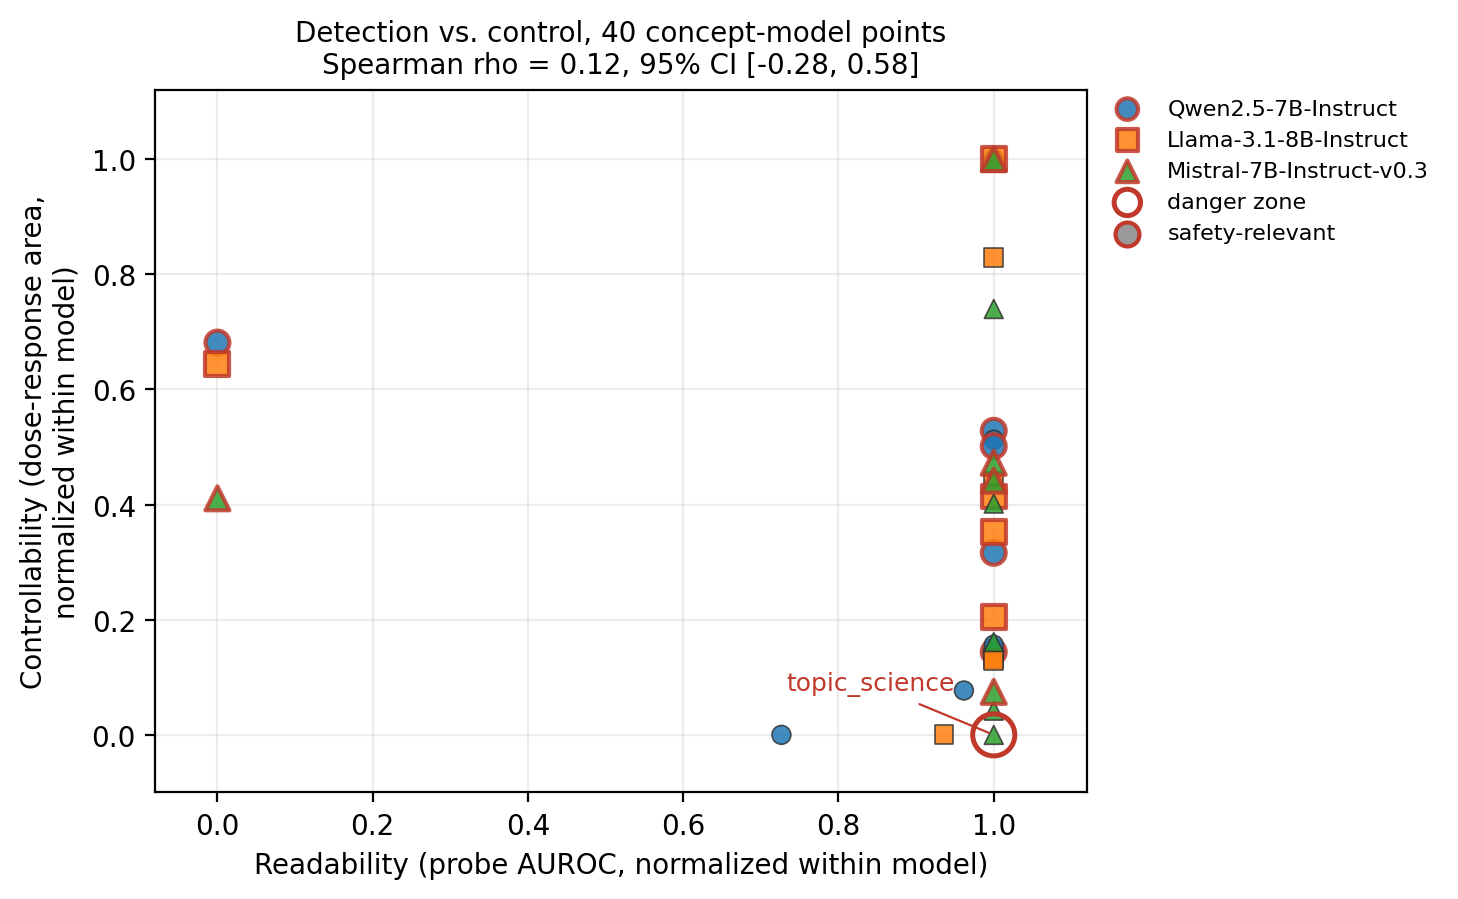
\includegraphics[width=0.82\linewidth]{fig1_gap_map.png}
  \caption{The gap map. Readability (probe AUROC) against controllability
  (dose-response area up to the fluency ceiling), both normalized within model.
  The high-readability, low-controllability corner is the danger zone; its two
  occupant (\texttt{topic\_science} on Mistral, circled) survived the six-method
  gauntlet. Readability is saturated: 24 of 30 points sit at AUROC $1.0$, which is
  why the correlation along this axis is uninformative rather than a null.}
  \label{fig:gapmap}
\end{figure}

\section{Absolute against directional controllability, per concept}
\label{app:absvsdir}

Figure~\ref{fig:directional} is the per-concept form of
Figure~\ref{fig:groundtruth}b. It was the previous version's main figure and
is kept because panel (b) gives the breakdown by concept that the summary
statistic in the main text does not.

\begin{figure}[htbp]
  \centering
  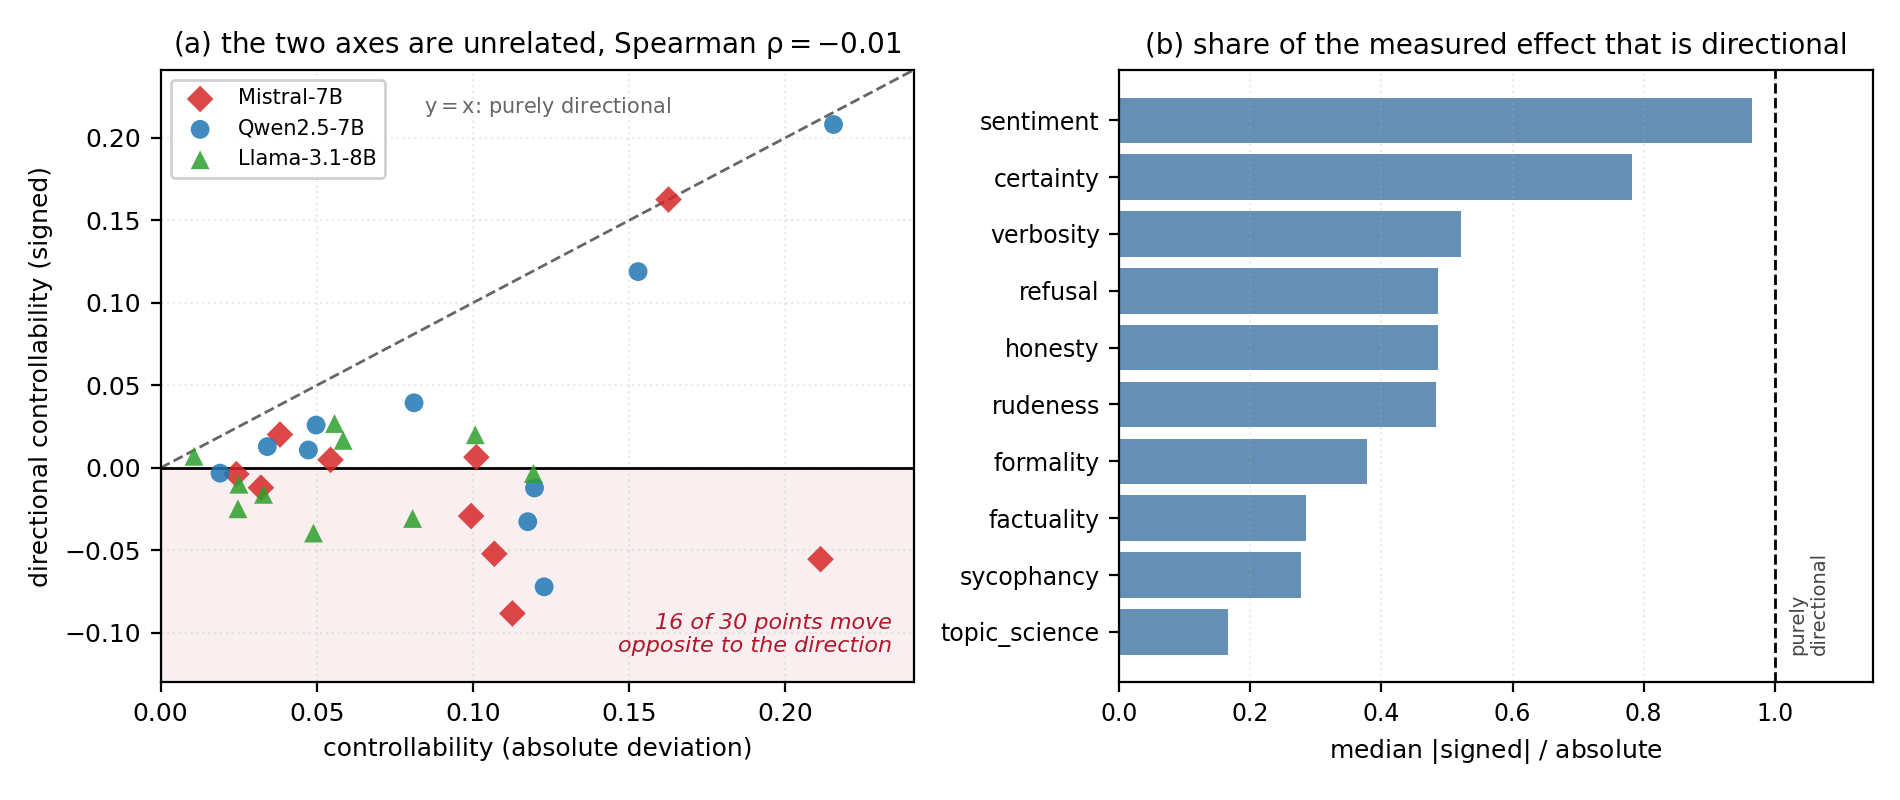
\includegraphics[width=\linewidth]{fig8_directional.png}
  \caption{Absolute against directional controllability on the judge-scored
  concepts. (a) The two summaries of the same curves are unrelated. Points below
  the line have a negative signed area, though none of those signs is resolved
  once prompt-level uncertainty is propagated (Appendix~\ref{app:signed}).
  (b) The share of each concept's measured effect attributable to directional
  movement, median over models.}
  \label{fig:directional}
\end{figure}

\section{Ground-truth concepts, per point}
\label{app:groundtruth}

Every ground-truth point, with the propagated interval on the signed area
and the same integral split by arm. The intended direction is positive
throughout by construction, so a negative entry is the intervention moving
the model against the direction it was estimated from, and a resolved
negative entry would be evidence the check is wrong where it is isolated, and
a finding where it is monotone. There is one, \texttt{gt\_question} on Llama.

\begin{table}[htbp]
  \caption{Directional controllability on the ground-truth concepts,
  whose readout is a rule over the generated string and whose intended
  direction is therefore known in advance. 26 of 40 points have an interval
  excluding zero and 25 of those are positive: where the sign is resolvable,
  steering almost always moved the model the way the direction was built to move
  it. The exception, \texttt{gt\_question} on Llama, is monotone in the wrong
  direction and is discussed in Section~\ref{sec:groundtruth}. \textbf{Pos} and \textbf{Neg} are the same integral over one arm,
  oriented so positive means the intended direction.}
  \label{tab:groundtruth}
  \centering
  \footnotesize
  \begin{tabular}{llccccc}
    \toprule
    Concept & Model & Abs & Signed & 95\% CI & Pos & Neg \\
    \midrule
    \texttt{gt\_digits} & Qwen2.5-7B & $0.009$ & $+0.008$ & $[-0.001, +0.051]$ & $+0.020$ & $+0.001$ \\
    \texttt{gt\_digits} & Mistral-7B & $0.001$ & $+0.001$ & $[-0.000, +0.002]$ & $-0.000$ & $+0.002$ \\
    \texttt{gt\_digits} & Llama-3.1-8B & $0.001$ & $-0.000$ & $[-0.003, +0.003]$ & $-0.001$ & $+0.001$ \\
    \texttt{gt\_digits} & Gemma-2-9b & $0.000$ & $+0.000$ & $[-0.000, +0.000]$ & $+0.000$ & $-0.000$ \\
    \texttt{gt\_french} & Qwen2.5-7B & $0.054$ & $+0.054$ & $[+0.033, +0.076]$\,\textbf{R} & $+0.174$ & $+0.000$ \\
    \texttt{gt\_french} & Mistral-7B & $0.057$ & $+0.057$ & $[+0.040, +0.075]$\,\textbf{R} & $+0.127$ & $+0.000$ \\
    \texttt{gt\_french} & Llama-3.1-8B & $0.040$ & $+0.040$ & $[+0.024, +0.058]$\,\textbf{R} & $+0.088$ & $+0.000$ \\
    \texttt{gt\_french} & Gemma-2-9b & $0.001$ & $+0.001$ & $[-0.000, +0.003]$ & $+0.001$ & $+0.000$ \\
    \texttt{gt\_length} & Qwen2.5-7B & $0.022$ & $-0.015$ & $[-0.051, +0.020]$ & $-0.030$ & $+0.021$ \\
    \texttt{gt\_length} & Mistral-7B & $0.011$ & $+0.003$ & $[-0.042, +0.049]$ & $-0.006$ & $+0.013$ \\
    \texttt{gt\_length} & Llama-3.1-8B & $0.013$ & $+0.012$ & $[-0.033, +0.058]$ & $+0.006$ & $+0.020$ \\
    \texttt{gt\_length} & Gemma-2-9b & $0.007$ & $-0.006$ & $[-0.036, +0.024]$ & $+0.000$ & $-0.015$ \\
    \texttt{gt\_uppercase} & Qwen2.5-7B & $0.017$ & $+0.017$ & $[-0.003, +0.046]$ & $+0.123$ & $+0.002$ \\
    \texttt{gt\_uppercase} & Mistral-7B & $0.183$ & $+0.181$ & $[+0.147, +0.215]$\,\textbf{R} & $+0.461$ & $+0.004$ \\
    \texttt{gt\_uppercase} & Llama-3.1-8B & $0.074$ & $+0.073$ & $[+0.028, +0.129]$\,\textbf{R} & $+0.183$ & $+0.004$ \\
    \texttt{gt\_uppercase} & Gemma-2-9b & $0.009$ & $+0.009$ & $[-0.002, +0.022]$ & $+0.028$ & $+0.005$ \\
    \bottomrule
  \end{tabular}
\end{table}

\section{Controls on the geometric test}
\label{app:controls}


Two alternative explanations for the sign of the primary test are ruled out
here, and a third is not.

\textbf{The fluency ceiling.} If output overlap indexed how lexical a direction
is, adding it might break fluency at low strength, truncate the usable
coefficient range, and shrink an integrated area for reasons that have nothing to
do with downstream sensitivity. Figure~\ref{fig:ceiling} and
Table~\ref{tab:ceiling} show this is not what happens. Overlap does not predict
where the ceiling falls, the ceiling rarely binds at all, and conditioning the
primary test on it changes nothing.

\begin{figure}[htbp]
  \centering
  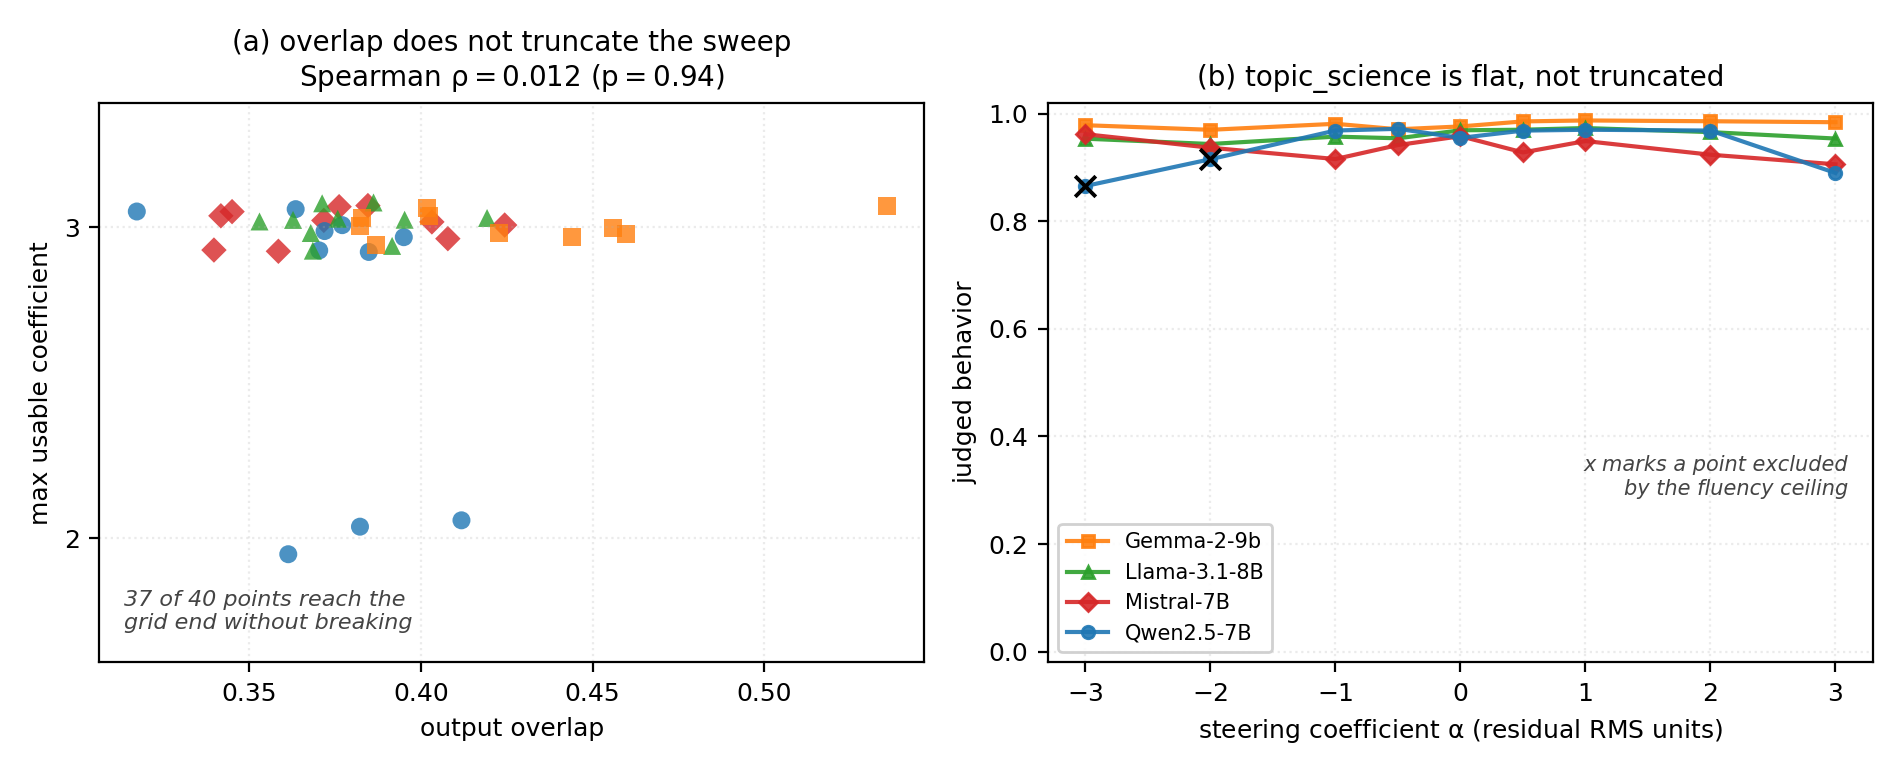
\includegraphics[width=\linewidth]{fig6_ceiling_control.png}
  \caption{The fluency ceiling does not explain the sign of the primary test.
  (a) Output overlap is unrelated to the largest usable coefficient, and almost
  every sweep reaches the end of the grid. (b) The \texttt{topic\_science} curves,
  the case that most invites the objection, are flat across the swept range rather
  than cut short by breakage.}
  \label{fig:ceiling}
\end{figure}

\begin{table}[htbp]
  \caption{The fluency ceiling does not explain the sign of the primary
  test. If output overlap made a direction lexical enough to break fluency early,
  it would shorten the usable coefficient range and shrink an integrated area
  mechanically. It does not: overlap is unrelated to where the ceiling falls, and
  conditioning the primary test on the ceiling as well as on readability leaves
  the estimate unchanged.}
  \label{tab:ceiling}
  \centering
  \footnotesize
  \begin{tabular}{lcc}
    \toprule
    Quantity & Statistic & $p$ \\
    \midrule
    \multicolumn{3}{l}{\emph{Does output overlap truncate the sweep?}} \\
    Overlap vs.\ max usable $|\alpha|$ & Spearman $-0.096$ & $0.61$ \\
    Overlap vs.\ number of usable grid points & Spearman $0.006$ & $0.98$ \\
    Max usable $|\alpha|$ vs.\ controllability & Spearman $0.019$ & $0.92$ \\
    \addlinespace
    \multicolumn{3}{l}{\emph{Primary test under wider control sets}} \\
    Partial $\rho$ $|$ readability & $-0.450$ & \\
    Partial $\rho$ $|$ readability, max usable $|\alpha|$ & $-0.450$ & \\
    Partial $\rho$ $|$ readability, ceiling, $n$ usable & $-0.435$ & \\
    \bottomrule
  \end{tabular}
\end{table}

\textbf{A single concept.} \texttt{topic\_science} holds the highest output
overlap and the lowest controllability on every model, so the estimate could be
one concept in disguise. Refitting with each concept removed in turn
(Figure~\ref{fig:loco}, Table~\ref{tab:loco}) leaves the estimate negative every
time. Dropping \texttt{topic\_science} weakens it most, to $-0.22$, so the concept
does carry more than its share without carrying the sign.

\begin{figure}[htbp]
  \centering
  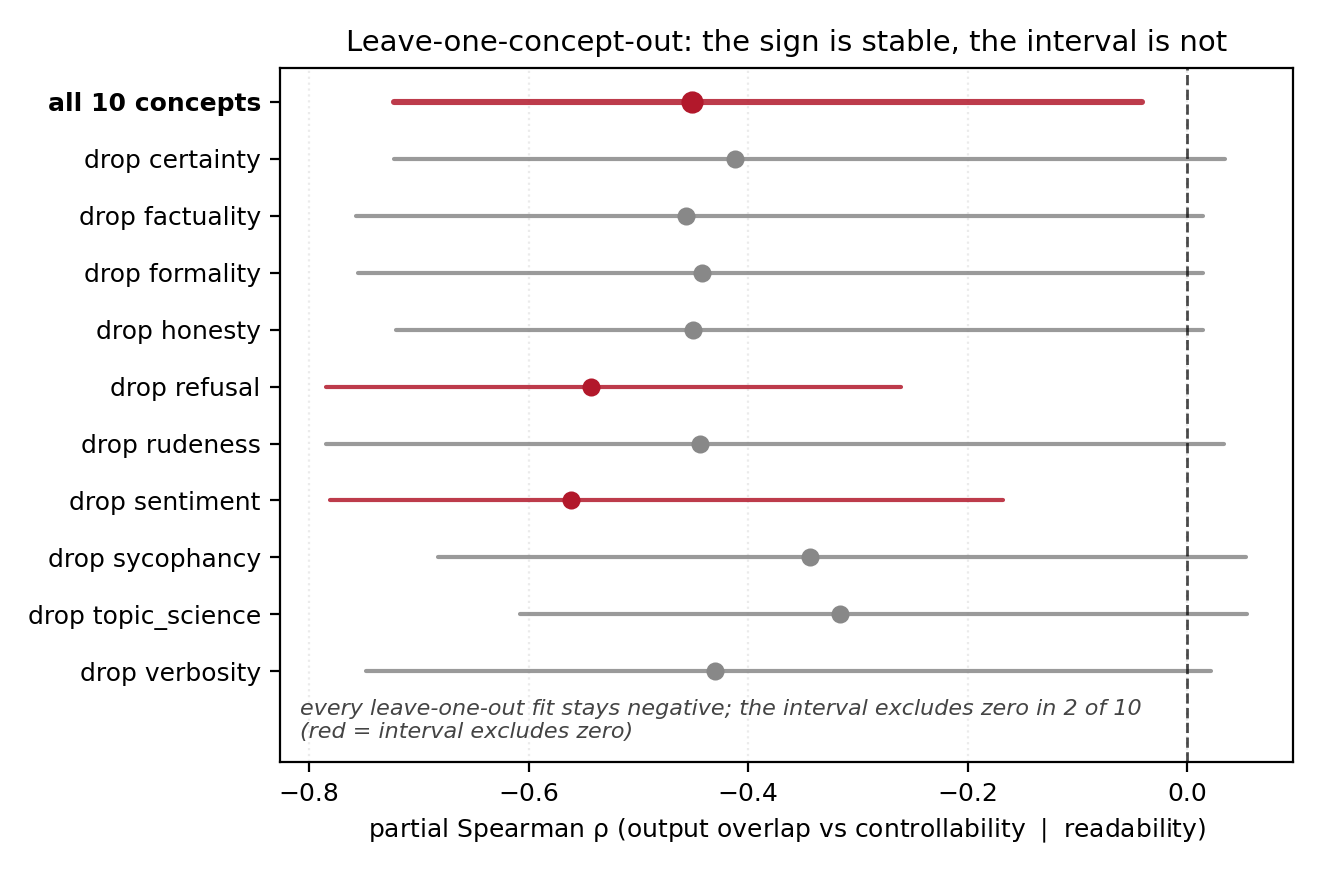
\includegraphics[width=0.86\linewidth]{fig7_loco.png}
  \caption{Leave-one-concept-out on the primary test. The point estimate stays
  negative in every refit; the interval excludes zero in two of ten, and on the
  retained sample it contains zero.}
  \label{fig:loco}
\end{figure}

\begin{table}[htbp]
  \caption{Leave-one-concept-out on the primary test. Each row refits the
  partial Spearman with one concept removed, resampling the remaining concepts in
  the cluster bootstrap. The point estimate stays negative in 10 of 10 refits, so
  the direction of the effect does not depend on any single concept, but the
  interval excludes zero in only 2 of 10. On the full retained sample the interval
  already contains zero. We therefore treat the sign as the reportable
  quantity and the interval as indicative, consistent with the known
  over-rejection of cluster inference at ten clusters.}
  \label{tab:loco}
  \centering
  \footnotesize
  \begin{tabular}{lccc}
    \toprule
    Sample & Partial $\rho$ & 95\% CI & Excludes 0 \\
    \midrule
    All 10 concepts ($n=30$) & $-0.450$ & $[-0.748, 0.038]$ & no \\
    \addlinespace
    drop \texttt{certainty} & $-0.433$ & $[-0.750, 0.114]$ & no \\
    drop \texttt{factuality} & $-0.435$ & $[-0.756, 0.120]$ & no \\
    drop \texttt{formality} & $-0.422$ & $[-0.770, 0.149]$ & no \\
    drop \texttt{honesty} & $-0.458$ & $[-0.757, 0.065]$ & no \\
    drop \texttt{refusal} & $-0.545$ & $[-0.795, -0.167]$ & yes \\
    drop \texttt{rudeness} & $-0.430$ & $[-0.768, 0.073]$ & no \\
    drop \texttt{sentiment} & $-0.528$ & $[-0.780, -0.030]$ & yes \\
    drop \texttt{sycophancy} & $-0.416$ & $[-0.735, 0.071]$ & no \\
    drop \texttt{topic\_science} & $-0.222$ & $[-0.544, 0.168]$ & no \\
    drop \texttt{verbosity} & $-0.400$ & $[-0.735, 0.142]$ & no \\
    \bottomrule
  \end{tabular}
\end{table}

\textbf{The metric.} The explanation that does survive is the change of summary
statistic, reported in Section~\ref{sec:directional} and
Appendix~\ref{app:directional}.

\section{Absolute and directional controllability, per point}
\label{app:directional}

Table~\ref{tab:directional} gives both summaries of every retained dose-response
curve, with the monotonicity of the curve alongside. The two summaries are
computed from identical data by identical code differing only in an absolute
value, so the disagreement between them is not attributable to sampling,
judging, or the ceiling.

The monotonicity column carries the harder result. If steering produced a small
but real directional effect, the sign of the monotonicity would agree across
models within a concept and only the magnitude would be small. Two of ten
concepts are same-signed on all three models. Under a null in which each model's
sign is an independent coin flip the expected count is $2 \cdot 2^{-3} \cdot 10 =
2.5$, so the observed agreement is what chance predicts. This is also what rules
out a sign-convention error in the direction estimate, which would have produced
agreement well above chance.

\begin{table}[htbp]
  \caption{Absolute versus directional controllability for all 30 retained
  points.
  \textbf{Abs} is the preregistered metric, the trapezoid of
  $|\text{behavior} - \text{baseline}|$ over the usable coefficient range.
  \textbf{Signed} is the same trapezoid without the absolute value, so it is
  positive only when positive coefficients raise the behavior and negative ones
  lower it. \textbf{Mono} is the Spearman correlation between coefficient and
  behavior along the sweep. 16 of 30 points have a negative signed area, meaning
  the intervention moved behavior against the direction it was built from, and the
  two metrics are uncorrelated (Spearman $-0.009$).}
  \label{tab:directional}
  \centering
  \footnotesize
  \begin{tabular}{llccc}
    \toprule
    Concept & Model & Abs & Signed & Mono \\
    \midrule
    \texttt{certainty} & Llama-3.1-8B & $0.049$ & $-0.039$ & $-0.86$ \\
    \texttt{certainty} & Mistral-7B & $0.113$ & $-0.088$ & $-0.73$ \\
    \texttt{certainty} & Qwen2.5-7B & $0.123$ & $-0.072$ & $-0.67$ \\
    \texttt{factuality} & Llama-3.1-8B & $0.058$ & $+0.017$ & $+0.05$ \\
    \texttt{factuality} & Mistral-7B & $0.032$ & $-0.012$ & $-0.72$ \\
    \texttt{factuality} & Qwen2.5-7B & $0.120$ & $-0.012$ & $-0.13$ \\
    \texttt{formality} & Llama-3.1-8B & $0.025$ & $-0.010$ & $-0.25$ \\
    \texttt{formality} & Mistral-7B & $0.099$ & $-0.029$ & $-0.17$ \\
    \texttt{formality} & Qwen2.5-7B & $0.034$ & $+0.013$ & $+0.49$ \\
    \texttt{honesty} & Llama-3.1-8B & $0.119$ & $-0.003$ & $+0.02$ \\
    \texttt{honesty} & Mistral-7B & $0.107$ & $-0.052$ & $-0.75$ \\
    \texttt{honesty} & Qwen2.5-7B & $0.081$ & $+0.039$ & $-0.10$ \\
    \texttt{refusal} & Llama-3.1-8B & $0.033$ & $-0.016$ & $-0.23$ \\
    \texttt{refusal} & Mistral-7B & $0.038$ & $+0.020$ & $+0.37$ \\
    \texttt{refusal} & Qwen2.5-7B & $0.047$ & $+0.011$ & $+0.20$ \\
    \texttt{rudeness} & Llama-3.1-8B & $0.056$ & $+0.027$ & $+0.58$ \\
    \texttt{rudeness} & Mistral-7B & $0.211$ & $-0.055$ & $-0.80$ \\
    \texttt{rudeness} & Qwen2.5-7B & $0.153$ & $+0.119$ & $+0.71$ \\
    \texttt{sentiment} & Llama-3.1-8B & $0.101$ & $+0.020$ & $+0.50$ \\
    \texttt{sentiment} & Mistral-7B & $0.163$ & $+0.163$ & $+0.98$ \\
    \texttt{sentiment} & Qwen2.5-7B & $0.215$ & $+0.208$ & $+0.79$ \\
    \texttt{sycophancy} & Llama-3.1-8B & $0.081$ & $-0.031$ & $-0.22$ \\
    \texttt{sycophancy} & Mistral-7B & $0.101$ & $+0.007$ & $+0.12$ \\
    \texttt{sycophancy} & Qwen2.5-7B & $0.118$ & $-0.033$ & $+0.38$ \\
    \texttt{topic\_science} & Llama-3.1-8B & $0.011$ & $+0.007$ & $+0.52$ \\
    \texttt{topic\_science} & Mistral-7B & $0.024$ & $-0.004$ & $-0.50$ \\
    \texttt{topic\_science} & Qwen2.5-7B & $0.019$ & $-0.003$ & $-0.50$ \\
    \texttt{verbosity} & Llama-3.1-8B & $0.025$ & $-0.025$ & $-0.93$ \\
    \texttt{verbosity} & Mistral-7B & $0.054$ & $+0.005$ & $+0.35$ \\
    \texttt{verbosity} & Qwen2.5-7B & $0.050$ & $+0.026$ & $+0.78$ \\
    \bottomrule
  \end{tabular}
\end{table}

\section{Directional controllability: intervals and arms}
\label{app:signed}

Per-prompt behavior scores are not retained in the result files, but every
coefficient carries a prompt-level bootstrap interval. We propagate those into
the signed area by Monte Carlo, drawing a behavior value per coefficient from a
normal whose standard error is the interval half-width over $1.96$, clipping to
$[0,1]$ because the judge emits a probability, and recomputing the area $4000$
times. Draws are independent across coefficients while the real scores share a
prompt set and are positively correlated, and correlated errors partly cancel in
a difference from baseline, so these intervals are conservative. That is the
safe direction for a claim that a sign is resolved.

3 of the 30 points have a signed area whose interval excludes zero, and all
3 are positive. 16 points have a negative signed area and none of them is
resolved, which is why this paper makes no claim about wrong-way movement.

\textbf{Pos} and \textbf{Neg} are the same integral computed over one arm of
the sweep, each oriented so that a positive value means the model moved the way
the direction intended. A concept with a genuine bidirectional effect scores
positive on both. 2 of 30 points do; 24 respond on one arm only. A signed area
near zero is therefore ambiguous between no directional effect and an effect
that is real but not monotone through the baseline, and these two columns are
what distinguish them.

\begin{table}[htbp]
  \caption{Signed controllability with a propagated 95\% interval, and the
  same quantity split by arm. \textbf{Abs} is the preregistered metric.
  \textbf{R} marks the three points whose sign is resolved. \textbf{Pos} and
  \textbf{Neg} are oriented so positive means the intended direction.}
  \label{tab:signed}
  \centering
  \footnotesize
  \begin{tabular}{llccccc}
    \toprule
    Concept & Model & Abs & Signed & 95\% CI & Pos & Neg \\
    \midrule
    \texttt{certainty} & Llama-3.1-8B & $0.049$ & $-0.039$ & $[-0.103, +0.026]$ & $-0.084$ & $-0.005$ \\
    \texttt{certainty} & Mistral-7B & $0.113$ & $-0.088$ & $[-0.183, +0.010]$ & $-0.187$ & $-0.008$ \\
    \texttt{certainty} & Qwen2.5-7B & $0.123$ & $-0.072$ & $[-0.172, +0.027]$ & $+0.060$ & $-0.217$ \\
    \texttt{factuality} & Llama-3.1-8B & $0.058$ & $+0.017$ & $[-0.055, +0.090]$ & $+0.077$ & $-0.047$ \\
    \texttt{factuality} & Mistral-7B & $0.032$ & $-0.012$ & $[-0.036, +0.011]$ & $-0.044$ & $+0.018$ \\
    \texttt{factuality} & Qwen2.5-7B & $0.120$ & $-0.012$ & $[-0.065, +0.041]$ & $+0.114$ & $-0.148$ \\
    \texttt{formality} & Llama-3.1-8B & $0.025$ & $-0.010$ & $[-0.060, +0.044]$ & $-0.036$ & $+0.016$ \\
    \texttt{formality} & Mistral-7B & $0.099$ & $-0.029$ & $[-0.118, +0.062]$ & $-0.125$ & $+0.099$ \\
    \texttt{formality} & Qwen2.5-7B & $0.034$ & $+0.013$ & $[-0.027, +0.060]$ & $-0.015$ & $+0.065$ \\
    \texttt{honesty} & Llama-3.1-8B & $0.119$ & $-0.003$ & $[-0.092, +0.088]$ & $+0.124$ & $-0.141$ \\
    \texttt{honesty} & Mistral-7B & $0.107$ & $-0.052$ & $[-0.139, +0.036]$ & $+0.057$ & $-0.173$ \\
    \texttt{honesty} & Qwen2.5-7B & $0.081$ & $+0.039$ & $[-0.060, +0.137]$ & $+0.080$ & $-0.021$ \\
    \texttt{refusal} & Llama-3.1-8B & $0.033$ & $-0.016$ & $[-0.071, +0.039]$ & $+0.013$ & $-0.054$ \\
    \texttt{refusal} & Mistral-7B & $0.038$ & $+0.020$ & $[-0.027, +0.068]$ & $+0.040$ & $+0.001$ \\
    \texttt{refusal} & Qwen2.5-7B & $0.047$ & $+0.011$ & $[-0.045, +0.067]$ & $-0.051$ & $+0.055$ \\
    \texttt{rudeness} & Llama-3.1-8B & $0.056$ & $+0.027$ & $[-0.099, +0.151]$ & $-0.033$ & $+0.097$ \\
    \texttt{rudeness} & Mistral-7B & $0.211$ & $-0.055$ & $[-0.168, +0.061]$ & $-0.299$ & $+0.165$ \\
    \texttt{rudeness} & Qwen2.5-7B & $0.153$ & $+0.119$ & $[+0.010, +0.226]$\,\textbf{R} & $-0.072$ & $+0.241$ \\
    \texttt{sentiment} & Llama-3.1-8B & $0.101$ & $+0.020$ & $[-0.016, +0.066]$ & $+0.140$ & $-0.084$ \\
    \texttt{sentiment} & Mistral-7B & $0.163$ & $+0.163$ & $[+0.071, +0.265]$\,\textbf{R} & $+0.011$ & $+0.368$ \\
    \texttt{sentiment} & Qwen2.5-7B & $0.215$ & $+0.208$ & $[+0.099, +0.320]$\,\textbf{R} & $-0.008$ & $+0.423$ \\
    \texttt{sycophancy} & Llama-3.1-8B & $0.081$ & $-0.031$ & $[-0.114, +0.055]$ & $+0.054$ & $-0.131$ \\
    \texttt{sycophancy} & Mistral-7B & $0.101$ & $+0.007$ & $[-0.074, +0.092]$ & $-0.096$ & $+0.117$ \\
    \texttt{sycophancy} & Qwen2.5-7B & $0.118$ & $-0.033$ & $[-0.115, +0.053]$ & $-0.107$ & $+0.102$ \\
    \texttt{topic\_science} & Llama-3.1-8B & $0.011$ & $+0.007$ & $[-0.003, +0.018]$ & $-0.003$ & $+0.018$ \\
    \texttt{topic\_science} & Mistral-7B & $0.024$ & $-0.004$ & $[-0.029, +0.023]$ & $-0.030$ & $+0.022$ \\
    \texttt{topic\_science} & Qwen2.5-7B & $0.019$ & $-0.003$ & $[-0.021, +0.014]$ & $-0.002$ & $-0.015$ \\
    \texttt{verbosity} & Llama-3.1-8B & $0.025$ & $-0.025$ & $[-0.060, +0.011]$ & $-0.024$ & $-0.035$ \\
    \texttt{verbosity} & Mistral-7B & $0.054$ & $+0.005$ & $[-0.036, +0.047]$ & $+0.064$ & $-0.052$ \\
    \texttt{verbosity} & Qwen2.5-7B & $0.050$ & $+0.026$ & $[-0.007, +0.060]$ & $-0.023$ & $+0.083$ \\
    \bottomrule
  \end{tabular}
\end{table}

\section{Judge validation and annotation setup in full}
\label{app:limits}

Agreement must be read within concept rather than pooled. Pooled agreement over
a multi-concept sheet mostly reflects that refusal text scores low and honesty
text scores high, which is trivially true when they answer different questions;
controllability is a within-concept quantity. We hand-labeled 100 generations
stratified across all ten concepts and compared three raters: a human, the fixed
logit judge, and a lexicon scorer.

On the positive control the judge tracks the human closely ($\alpha = 0.76$ for
sentiment), so the instrument behaves as intended where behavior varies. On
\texttt{topic\_science} the judge's spread across sampled generations is $0.02$,
below the human's $0.05$, so the near-zero controllability that places this
concept in the danger zone is unlikely to be a judge artifact.

Two features of the annotation setup bear on how much weight the validation
carries. The labels come from a single annotator, so no inter-annotator
agreement can be computed and the reported figures rest on that annotator's
judgment; the ten repeated items give intra-rater reliability only. Against
that, the annotator was blind to condition: the labeling sheet carries the
generation, its concept and the scoring question, and does not record which
model produced the text or at what steering strength, so the labels cannot have
been shaped by knowing whether an item came from a steered or unsteered
condition. The annotator was not blind to the hypothesis under test, which a
second independent rater would address and which we did not do.

The exception is \texttt{refusal}. The human scored all ten sampled outputs
identically, while the judge spread them over $0.16$. That interval is the sole
reason \texttt{refusal} misses the danger-zone criterion. We record this rather
than argue from it, since determining where \texttt{refusal} lies would require
re-measurement with a better-validated judge.

A second judge cannot be run from the released artifacts alone. The result files
cache two generations per coefficient per point, 720 in total, which is enough
to inspect behavior but not to re-score the curves. Re-judging requires
regenerating, which is the main cost of the experiment.

Section~\ref{sec:directional} rules out judge noise as the explanation for the
directional result specifically: wrong-way movement appears at the same rate in
the four concepts with near-zero human variance as in the six without. That
argument concerns the sign of the effect and does not rehabilitate the
magnitudes on those four concepts.

\section{Corrections, retractions and the replication sequence}
\label{app:corrections}

This appendix holds the detail behind four statements the main text makes
briefly. Each concerns an error of ours, and in each case the error ran in the
direction that favored a claim we were making.

\textbf{The per-coefficient interval.} The signed-area interval is propagated
from an interval on the mean behavior at each coefficient. An earlier version
used the $2.5$th and $97.5$th percentiles of the individual generation scores
instead: the spread of the generations rather than an interval for their mean.
The two differ by roughly $\sqrt{n}$. On a judge readout, whose scores spread
across $[0,1]$, the stored interval sat near $[0,1]$ whatever the mean, about
three times too wide at thirty prompts. On a sparse rule readout, where most
generations score exactly zero, both percentiles collapsed onto zero. A
percentile interval also cannot narrow as prompts are added, so an earlier
reading of the six-versus-thirty prompt comparison, that the judge's intervals
failed to tighten, was uninformative by construction. Recomputed from
per-generation scores, the rule-scored resolution count on identical data moves
from 6 of 40 to 26 of 40. The prompt-level bootstrap behind absolute
controllability was always an interval for the mean and is unaffected, as is
every quantity that does not use a per-coefficient interval.

\textbf{Six prompts against thirty.} With the judge, grid and models held fixed
on four concepts, mean interval width falls from $0.175$ to $0.099$, a ratio of
$0.57$ against the $1/\sqrt{5} = 0.45$ that pure sampling predicts. The point
estimates move far more than their intervals: median magnitude falls by $0.028$
and 7 of 16 signs flip. \texttt{refusal} on Gemma goes from $+0.139$ to $+0.015$
and \texttt{topic\_science} on Mistral from $-0.201$ to $+0.043$.

\textbf{The replication sequence.} Several versions of the activation-addition
replication preceded the one reported, and between them they carried four
faults, found in this order. The first version decoded greedily against a
sampling result; greedy GPT-2-XL falls into a repetition loop, and a
coefficient-scale nudge cannot move an argmax path, so coefficients from $+1$ to
$+15$ produced text identical to the unsteered completion. The second swept
coefficients in residual-RMS units on a unit-normalized direction, while the
published coefficient multiplies the raw activation difference, whose norm was
about $175$; the grid was never shown to contain the published operating point.
Those two were fixed together. The next version used a single pooled last-token
vector added at every covered position, where activation addition differences
the padded prompts position by position and adds row $i$ at position $i$. The
version after that added a correctly built vector at layer $6$, recorded from
memory, where the paper states layer $16$. A
diagnostic sweep over spellings of the contrast, run at the wrong layer, pointed
at capitalization and was misleading: at layer $16$ every three-token spelling
reproduces the effect, including the capitalized one. The positive control,
added after the first failure, failed on every later version until the layer was
corrected, and passed then; no null from any earlier version was reported.

\textbf{The positive control and Gemma.} An earlier version applied a weaker
control: on six prompts Llama's signed sentiment area was unresolved at $+0.083$
and was retained on a judgment call, while Gemma was withheld because its
estimate was negative. Neither premise survived the corrected measurement, and
the strict control is now applied throughout. That version also reported that
Gemma's ground-truth controllability sat five to eight times below the other
models and read this as Gemma withholding its concepts. Under the four-layer
band its median was $0.0040$ against $0.0195$ to $0.0342$; but banded
controllability is a maximum over four layers, and at a single layer on the same
four concepts Gemma's median is above Llama's and Qwen's. Across all ten concepts
absolute area does not separate models at all (Kruskal--Wallis $H=0.33$,
$p=0.95$). The claim is withdrawn.

\textbf{The matched pair.} \texttt{gt\_lowercase} and \texttt{gt\_uppercase} read
the same property from opposite ends, so the room available to an absolute
deviation is $0.97$ for both. Absolute areas: Llama $0.0058$ and $0.0044$, Qwen
$0.0030$ and $0.0031$, Mistral $0.0254$ and $0.0205$, Gemma $0.0415$ and
$0.0043$. The first three agree despite baselines $0.94$ apart. Gemma's tenfold
difference is a concept-by-model interaction that matched room cannot explain.

\textbf{A sign-convention check.} \texttt{certainty} responds negatively on every
model in the main study, which is what an inverted direction would produce. Its
stimuli are correctly signed, and a systematic polarity error would show many
concepts agreeing in sign across models rather than the two of ten chance
predicts.

\section{Failure modes encountered, and how they were caught}
\label{app:failures}

Several measurement errors in this study would have produced a plausible-looking
result rather than an obvious crash. We record them because each one is a
failure mode a replication could repeat, and because the specific pattern is
instructive: in every case the corrupted quantity was pushed toward the value
the danger-zone criterion selects for, so the error would have manufactured
support for our own hypothesis.

\textbf{A judge returning a constant.} An early sweep produced controllability
exactly $0.000$ on the positive control with no parse failures. A judge that
emits the same score for every generation yields a perfectly flat dose-response
curve, which is indistinguishable from a concept that steering cannot move. The
harness now records whether a sweep returned a single distinct score and
excludes such points, because a warning is not sufficient when the number being
warned about is the number the finding is defined by.

\textbf{Prompting an instruction-tuned model without its chat template.} The
same early sweep fed raw instructions to instruct models, which continued the
instruction rather than following it. The resulting text was uniform enough
that the judge scored it identically throughout, again producing a flat curve.
Steering itself was never broken; the stimulus was.

\textbf{Applying danger-zone thresholds to normalized values.} Both axes are
min-max normalized within model for the correlation and the figure, which is
necessary because raw AUROC and raw dose-response area are not comparable across
models. Applying the danger-zone thresholds after that normalization is not:
min-max normalization guarantees that some point sits at each extreme, so
thresholding normalized values manufactures a danger-zone occupant out of pure
scatter. The thresholds are therefore applied to raw values, and a test
constructed from scatter confirms that no occupant appears.

\textbf{A fluency ceiling that admitted the point that breached it.} The
original ceiling walked outward by absolute coefficient against a single scalar,
so a breach at one sign could leave the opposite sign's breaching point inside
the usable set. The ceiling now marks each point on its own perplexity and
repetition and closes over each sign separately, and the confidence interval is
computed on the same usable set as the point estimate rather than on a magnitude
threshold.

\textbf{Selecting the probe layer on test AUROC.} Layer selection originally
maximized test AUROC and then reported that same maximum as readability. Layer
choice now happens on a validation family split disjoint from both train and
test.

\textbf{A verdict rule that ignored the sign of its own result.} The primary
test's reporting logic checked whether the estimate was in the predicted
direction only when its magnitude exceeded $0.7$. Our result is moderate
($-0.45$) with an interval excluding zero on the side opposite the prediction,
and it therefore fell through to a branch that described it as suggestive
support. A wrong-signed result whose interval excludes zero is evidence against
the hypothesis, and the reporting is now sign-aware at every magnitude.

\textbf{A hand-labelling sheet with no within-concept variance.} The first
judge-validation sheet was drawn as the first hundred generations in curve
order. Because steering frequently leaves output unchanged at adjacent
coefficients, 56\% of its rows were duplicates, four of ten concepts were absent
including the positive control, and the sampled generations spanned too little
of the sweep to exhibit within-concept variation. Agreement computed on it read
$+0.573$ pooled against $+0.022$ within concept. The sampler now deduplicates,
allocates across concepts round-robin, and spreads picks across the coefficient
range.

The common thread is that a metric can be wrong in a direction that flatters the
hypothesis without failing loudly. Every quantity reported here is covered by
tests that run the metric against synthetic data with a planted ground truth, so
a metric that returns a wrong number fails a test rather than reaching a figure;
the two reporting errors above were both found that way.

\end{document}
